\documentclass{article}
\usepackage{tmlr}
\usepackage[utf8]{inputenc}
\usepackage{amsmath,amssymb,amsthm}
\usepackage{graphicx}
\usepackage{booktabs}
\usepackage{subcaption}
\usepackage{algorithm}
\usepackage{algpseudocode}
\usepackage{xcolor}
\usepackage[hidelinks]{hyperref}
\usepackage{cleveref}

\graphicspath{{../figures/}}

\newtheorem{lemma}{Lemma}
\newtheorem{proposition}{Proposition}
\newtheorem{definition}{Definition}
\newtheorem{assumption}{Assumption}
\newtheorem{remark}{Remark}

\newcommand{\dhat}{\hat{\Delta}}
\newcommand{\Dw}{\Delta_W}
\newcommand{\rmax}{r_{\max}}
\newcommand{\sigd}{\sigma_{\Delta}}
\newcommand{\pizero}{\pi_0}

\begin{document}

\title{Bouncer: Competence Auditing for\\ Set-Local Learned Microarchitectural Controllers}

\author{Anonymous authors}

\maketitle

\begin{abstract}
Learned microarchitectural controllers can outperform fixed heuristics on average
yet regress under workload shift or adversarial steering. We present
\textbf{Bouncer}, a runtime monitor and trust gate that measures \emph{realized
competence}: it secretly set-duels a learned controller against a vetted fallback
on hidden, per-epoch-reshuffled sets and gates the controller when its measured
advantage falls below a threshold.

Under bounded rewards, secret uniform sampling, and explicit assumptions on
detection, re-trust, and false alarms, Bouncer bounds expected window-normalized
regret over audited declared domains by three terms: fully-open detection and
re-trust windows, audit exposure proportional to the secret dueling fraction and
drop duration, and false-alarm switching. A per-domain result gives an
expectation-level mimicry floor. For a truly degrading strategy whose conditional
window mean is at most $\tau-\epsilon$, independence of per-window estimates given
the strategy yields an exponentially decreasing probability of sustained realized
evasion. The result gives no single-window guarantee and does not cover
sub-resolution harm.

Given representative within-domain sampling, faithful auditing requires two
controller-side properties. First, reward must be \emph{set-local},
so a decision and its outcome can be attributed to the same dueling pool. Cache
replacement satisfies this spatial condition; prefetching does not because a
prefetch can benefit a different set. Second, the policy contrast must be
\emph{reseed-identifiable}, so reshuffling leaders does not erase the measured
advantage. A stateless reward is sufficient but not necessary: a stateful reward
with state-invariant contrast remains auditable. We argue that each condition is
necessary and demonstrate both boundaries; a full sufficiency theorem remains
future work.

In a released, seeded synthetic harness satisfying both conditions, the estimator
tracks ground truth ($R^2{=}0.997$), the attacked steady-state floor remains within
$0.64\%$ of the fallback, detection takes two audit windows at the operating point,
and the clean-workload tax is $0.35\%$. Across $50$ seeds, Bouncer detects all
mimicry attacks ($50/50$; Wilson $95\%$ lower bound $0.93$), whereas an
input-distribution monitor detects none ($0/50$; upper bound $0.07$). A leak
ablation shows detection collapse between $0.6$ and $0.8$ leaked assignment
fraction, while a slow-bleed attack exposes the finite-resolution limit.

ChampSim experiments serve as boundary studies rather than full-system validation:
prefetch reward is not set-local, and secret reseeding confounds a path-dependent
cache-replacement reward. An illustrative 16-bit representation of the released
Tier-A dimensions requires about $406$\,bytes ($0.15\%$ of a 256\,KB static
random-access memory). Register-transfer-level area, energy, and timing remain
unmeasured.
\end{abstract}

\section{Introduction}
Modern processors increasingly hand small \emph{learned} models control of
decisions that used to be made by fixed, hand-tuned rules. Consider the
\emph{cache}---a small, fast memory that holds recently or soon-to-be-used
data so the processor rarely waits on slow main memory. Two decisions dominate a
cache's performance: which data to \emph{prefetch} (fetch early, before it is
asked for) and which block to \emph{evict} when the cache is full
(\emph{replacement}). Learned versions of both now beat the classic
heuristics---a reinforcement-learning prefetcher~\citep{bera2021pythia}, an
imitation-learned replacement policy~\citep{jain2016hawkeye,shi2019glider}---and
similar learned controllers are arriving for memory scheduling and branch
prediction~\citep{ipek2008selfoptimizing,jimenez2001perceptron}. The tempting move
is to ship them and trust the average: they were validated to win, so let them
run.

\begin{figure}[t]\centering
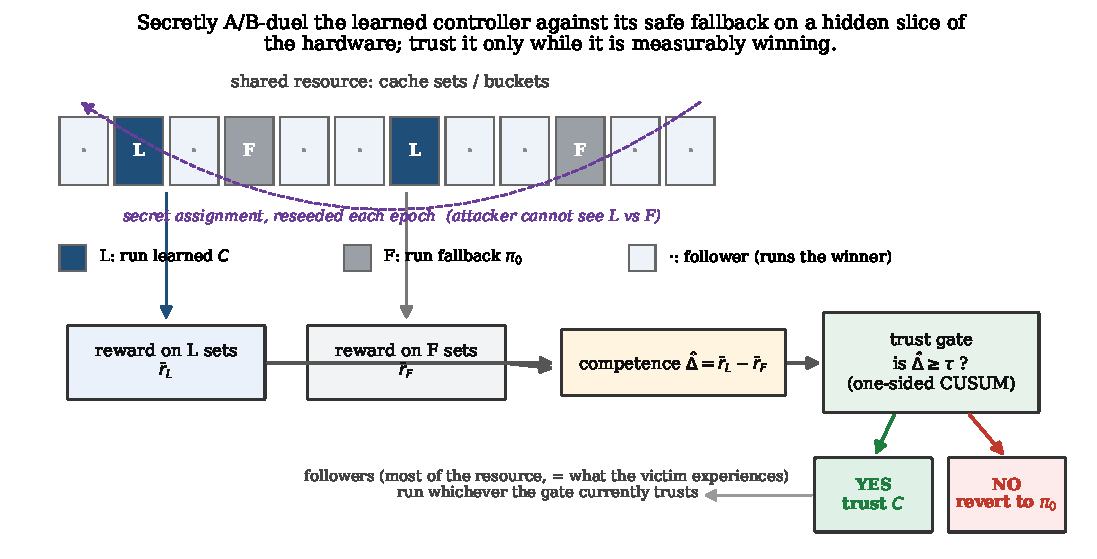
\includegraphics[width=\linewidth]{concept.pdf}
\caption{\textbf{Secretly A/B-duel the learned controller against its safe
fallback on a hidden slice of the hardware; trust it only while it is measurably
winning.} A few randomly chosen \emph{sets} (address buckets in the cache) run the
learned controller, a few run the fallback, and the assignment is a hardware
secret reshuffled each epoch (a fixed interval). Because the winner is
\emph{measured}, expected regret is bounded under the stated assumptions. With
representative within-domain sampling, an intact secret, and temporal independence,
sustained audit evasion by a degrading strategy becomes exponentially unlikely; no
single-window guarantee is claimed.}
\label{fig:concept}
\end{figure}

``Wins on average,'' though, is a property of the workloads a controller was
validated on, and it does not travel. On a new program or a new execution phase a
learned controller can quietly become \emph{worse} than the simple heuristic it
displaced---a silent regression that aggregate performance counters never flag.
Worse still, a shared on-chip controller is exercised by \emph{every} program on
the core, so a hostile co-running program can \emph{steer} it: craft memory
accesses that push the controller into its bad regime while keeping the aggregate
counters looking normal~\citep{guo2022adversarialprefetch,evtyushkin2018branchscope}.
Nothing in a deployed system checks, at runtime, whether the learned controller is
still earning its keep. The obvious check---watch the controller's \emph{inputs}
for distribution shift---is both insufficient and unsafe: an attacker can hold the
input statistics in-distribution while wrecking the controller's behavior (a
\emph{mimicry} attack), and an input monitor is blind to that by construction.

We instead check the thing that actually matters: \emph{realized competence}, whether
the learned controller is beating the fallback \emph{right now}---and we show this can
be done cheaply, provably, and without trusting the inputs. The mechanism
(\Cref{fig:concept}) builds on the fact that a cache slices its storage into many
\emph{sets} (address buckets that each memory address maps into). It repurposes
\emph{set-dueling}---running two candidate policies on different sets and comparing
them---a technique already in commercial caches: we secretly dedicate a randomly
chosen handful of sets to run the learned controller and another handful to run the
safe fallback, compare the reward they earn, and let the rest of the cache follow
the current winner. If the learned controller stops winning, the gate reverts to
the fallback. Measurement yields an expected-regret bound. Secrecy supplies a
different property: under the per-domain sampling and temporal assumptions of
\Cref{prop:mimicry}, a degrading strategy is exponentially unlikely to evade the
audit for many consecutive windows. A single realized window has no such
guarantee.

The central finding is \emph{where this works and where it does not}. Secret
set-dueling can attribute reward to the right policy only if that reward is
\emph{set-local}: the outcome of a decision made on a set is realized on that same
set. Cache \emph{replacement} is set-local---an eviction on a set is scored by the
hits and misses on that set---and is the clean case. \emph{Prefetching is the
instructive boundary}: a prefetch triggered on one set benefits a \emph{different}
set, so no per-set reward captures it, and we confirm on a real simulator that not
even the controller's own reward rescues the audit (\Cref{sec:eval-champsim}). A
second condition surfaces in the real-trace simulator study, and it is \emph{not} statelessness. The
secret reshuffle erases any long-run, policy-specific state a reward accumulates, so
what the audit needs is that the policy \emph{contrast}---the C-minus-fallback
advantage---survive that erasure: the reward must be \emph{reseed-identifiable}. A
(near-)stateless reward is the clean way to get this, but not the only way: we show
an additive-warmup reward that is \emph{stateful} yet stays auditable because its
contrast is state-invariant, and a multiplicative-warmup reward (the cache case) that
fails because its contrast scales with the state the reshuffle destroys. Together,
set-locality and reseed-identifiability are the two conditions we identify as \emph{governing}
which controllers this kind of audit can certify: we argue each is necessary and demonstrate the
boundary on real and synthetic controllers, leaving a complete sufficiency theorem to future
work---the paper's organizing result, with prefetching and one named security limitation as its
honest boundaries.

\paragraph{Contributions.}
\begin{enumerate}
\item \textbf{Two conditions for faithful auditing} (\Cref{sec:setting}, \Cref{def:setlocal},
\Cref{rem:stateless}): set-locality and reseed-identifiability of the policy contrast
are two conditions we identify as governing when secret set-dueling can faithfully audit a
learned controller---we argue each is necessary and demonstrate the boundary, leaving a full
sufficiency theorem to future work (statelessness is one sufficient special case of the second). On a
real simulator we probe the boundary one trace at a time: replacement is set-local
(and we expose where its stateful reward is not reseed-identifiable), while
prefetching is not set-local.
\item \textbf{The mechanism} (\Cref{sec:tierb}): a counterfactual-free competence
estimator that repurposes the set-dueling substrate~\citep{qureshi2007dip,jaleel2010rrip}
from \emph{choosing} a policy to \emph{trusting} one, gated by a change detector and a
four-state trust machine, all off the memory-access critical path (out of the
latency-critical access loop).
\item \textbf{Two guarantees} (\Cref{sec:guarantees}): an \emph{expected}-regret safety floor
(\Cref{lem:floor})---bounding the mean regret against the fallback---tied to the run-length theory
of the detector, and a mimicry-resistance result (\Cref{prop:mimicry}) purchased by
the secrecy and per-epoch independence of the sampler---an expectation-level floor
plus an exponentially-decaying bound on \emph{sustained} realized evasion; together
with an honestly named limitation, a slow-bleed attacker who stays below the audit's
resolution and evades it.
\item \textbf{A cheap, released design} (\Cref{sec:overhead,sec:eval}): a two-tier
microarchitecture whose auditor fits in a few hundred bytes and sits off the cache's
critical path, evaluated by a synthetic harness that validates the guarantees and a
study on a real cycle-accurate CPU simulator (ChampSim) that both demonstrates the
downside cap and exposes the reward-localizability boundary.
\end{enumerate}
\noindent We are explicit throughout (\Cref{sec:method,sec:disc}) about what is
\emph{proven}, what is \emph{measured} in a controlled synthetic harness---whose
load-bearing assumptions (bounded reward, a partitionable resource, and a secret uniform
sampler, A1--A6; plus, for faithful auditing, set-locality and reseed-identifiability) are
exactly those the guarantees rest on---and what is \emph{demonstrated} on a real simulator.


\section{Formal setting}\label{sec:setting}
A learned controller $C$ is invoked at decision points $t=1,2,\dots$. At each
point it observes microarchitectural state $x_t\in\mathbb{R}^d$ (the hardware's
internal counters and flags), emits action $a_t\in\mathcal{A}$, and receives a
bounded reward $r_t\in[0,\rmax]$ after a short horizon. Examples include prefetch
hit$\times$timeliness, cache hit, a normalized latency-saving reward, and branch
correctness. The controller was trained or validated on a distribution $D_{val}$
of $(x,a,r)$. A fixed safe fallback $\pizero$ has a known, attack-resistant
competence floor.

\begin{definition}[Competence advantage]
Index audit windows by $w$, and let $W_w$ be the decision points in window $w$.
For policy $\pi$, define the normalized window reward
$\bar r_w^\pi:=|W_w|^{-1}\sum_{t\in W_w}r_t^\pi$. The competence advantage is
$\Delta_w:=\bar r_w^C-\bar r_w^{\pizero}$.
\end{definition}
$r_t^{\pizero}$ is counterfactual---one cannot run both policies on the same
decision---which is the central estimation challenge \Cref{sec:tierb} solves.
Unless stated otherwise, the CUSUM, gate, and regret bound below use audit-window
units: rewards are the normalized $\bar r_w$, and durations are numbers of windows.

\begin{definition}[Off-policy condition]
The system is \emph{off-policy} in window $w$ iff $\Delta_w<\tau$ for a trust threshold
$\tau\ge 0$. $\tau{=}0$ means ``learned no longer beats the floor''; $\tau{>}0$
gives margin and hysteresis.
\end{definition}

This one scalar unifies the two threats: an adversarial push toward $C$'s
decision boundary and a benign distribution shift both manifest as $\Delta_w$ falling.
The auditor detects the condition; a lightweight triage (\Cref{sec:triage})
guesses the cause to pick the response.

\begin{definition}[Set-locality]\label{def:setlocal}
Let the resource be partitioned into dueling sets $\{s\}$. A controller is
\emph{set-local} if the reward $r_t$ for a decision made on set $s$ is realized on
set $s$ (so it can be attributed to $s$'s pool). This is the \emph{spatial
attribution} property: each pool mean aggregates only rewards its own policy earned.
Set-locality alone does \emph{not} make $\dhat=\bar r_L-\bar r_F$ a faithful
competence estimate---faithfulness additionally requires the reseed-identifiability
condition of \Cref{rem:stateless} (a set-local, stateful reward can still defeat the
reseeded audit, as the real replacement study shows).
\end{definition}

Set-locality prevents $\dhat$ (\Cref{sec:tierb}) from mixing rewards earned by
different sets. It is necessary for spatial attribution, but not sufficient for a
faithful competence estimate. Cache \emph{replacement} (deciding which cached block to evict) satisfies the spatial-attribution requirement exactly
(the eviction on $s$ is rewarded by hits/misses on $s$); PC-indexed predictors
satisfy it too---though, as \Cref{rem:stateless} and \Cref{sec:eval-champsim}
show, replacement's reward is \emph{stateful}, so a secret reseeded audit does
not recover a faithful $\dhat$ there at per-window grain; \emph{prefetch}
violates it (a prefetch on $s$ benefits a different set $s'$), and we show in
\Cref{sec:eval-champsim} that no per-set reward---not even the controller's own---
recovers a faithful $\dhat$ for it. We therefore present Bouncer as a mechanism for
the \emph{set-local} class, with replacement as the canonical instance and
prefetching as the demonstrated boundary.

These are controller-side attribution conditions, not a substitute for statistical
representativeness. The pool estimator targets the decision-weighted $\Delta_w$
only when the sampled sets represent the domain's traffic, or when the estimator is
weighted accordingly. \Cref{prop:mimicry} states this requirement as within-domain
exchangeability up to bias $\beta$; the synthetic harness enforces it by drawing the
same number $m$ of decisions per set. Without such a premise, even a stateless,
set-local reward can yield a biased $\dhat$ under skewed traffic.

\begin{definition}[Reseed-identifiability]\label{rem:stateless}
Let $\mathcal{D}_{rs}$ denote the short-run state distribution induced by
reseeding leaders. Given representative sampling, define the signed reseed contrast
$\hat g:=\mathbb{E}_{s\sim\mathcal{D}_{rs}}[r_C(s)-r_F(s)]$. A set-local audit is
\emph{reseed-identifiable} at threshold $\tau$ when reseeding preserves the trust
decision,
\[
\mathrm{sign}(\hat g-\tau)=\mathrm{sign}(\Delta-\tau),
\]
with enough separation from $\tau$ for the detector to resolve the decision.
\end{definition}

Stateful reward can violate this condition: a cache hit on set $s$ depends on the
blocks retained by earlier evictions, while reseeding repeatedly returns sampled
sets to short-run state. The signed definition matters because a contrast moved to
the wrong side of $\tau$ would reverse the gate.

Statelessness removes this state-history failure mode, but it does not remove the
representativeness requirement above. Nor is statelessness necessary. An additive
warmup $r_C(k)=\mu_C-b e^{-ck}$, $r_F(k)=\mu_F-b e^{-ck}$ has the state-invariant
contrast $\mu_C-\mu_F$ and remains identifiable. A multiplicative warmup
$r_C(k)=\mu_C(1-e^{-ck})$ has contrast
$(\mu_C-\mu_F)(1-e^{-ck})$, which reseeding attenuates (\Cref{sec:eval-e3warmup}).
The balanced, independent synthetic harness satisfies both representativeness and
reseed-identifiability. Real cache replacement is set-local but exhibits the
multiplicative failure: reseeded estimates collapse while fixed leaders recover the
gap (\Cref{sec:eval-champsim}).

\section{Threat model}\label{sec:threat}
\textbf{In scope.} A co-located tenant/process sharing $C$ that issues arbitrary
memory accesses and knows the Bouncer design (Kerckhoffs). Its goal is denial of
service (DoS) or steering $C$ into a covert or side channel.

\textbf{Out of scope.} Physical and fault attacks, direct weight tampering, and
online-learning poisoning are outside the base model, which fixes weights at
deployment. GATED freezes learning and stops further updates, but it neither
repairs a policy poisoned during TRUSTED operation nor prevents PROBING from
restoring it. Defending learned \emph{state}, rather than the steered-input threat
studied here, remains future work.

\textbf{The secret.} A hardware random-number generator (RNG) supplies a
per-epoch seed that assigns the dueling sets. The assignment is not exposed
through an architectural channel.

\textbf{The adaptive adversary (headline).} The headline \emph{mimicry} attack
keeps Tier-A's input statistics in-distribution while degrading $C$. Measuring
realized competence, rather than inputs, is what exposes this attack; the
$50/50$-versus-$0/50$ experiment isolates that distinction (\Cref{sec:eval-p4}).
Secrecy addresses a separate move: an attacker who identifies the dueling sets can
spare them and pass the audit. The leak ablation measures this secrecy dependence.

\textbf{Realizability---what we do and do not demonstrate.} Bouncer's guarantees
bound the cost of \emph{any} in-domain competence degradation \emph{however it
arises}: benign distribution shift or adversarial steering are the same scalar
event ($\Delta_w{<}\tau$) to the auditor. We realize the mimicry/steering adversary in
the synthetic competence harness, where the latent stress~$u$ is the controllable
knob; the real-ChampSim study (\Cref{sec:eval-champsim}) drives the auditor with an
\emph{injected, controlled, labelled} competence degradation---a deliberately-bad
eviction policy active on a known phase---\emph{not} a demonstrated end-to-end
real-silicon steering attack. Whether a co-located tenant can realizably steer a
\emph{specific deployed} controller to sub-resolution harm on real silicon, rather
than in our harness, is \emph{not established here and is future work}; the
defense's guarantee is degradation-source-agnostic, so the harness's injected
degradation is a faithful stand-in regardless of how a real degradation would be
induced.

\section{Architecture}\label{sec:arch}
Bouncer is two-tier because cheap input signals are spoofable and direct
competence confirmation costs more. Cheap, always-on tripwires (Tier-A) raise the
duty cycle of a competence confirmer (Tier-B; \Cref{fig:arch}). The estimator and
gate logic are epoch-grained and off the cache-access critical path; the proposed
per-access pool-tag lookup and output multiplexer are accounted for separately in
\Cref{sec:overhead}.

\begin{figure}[t]
\centering
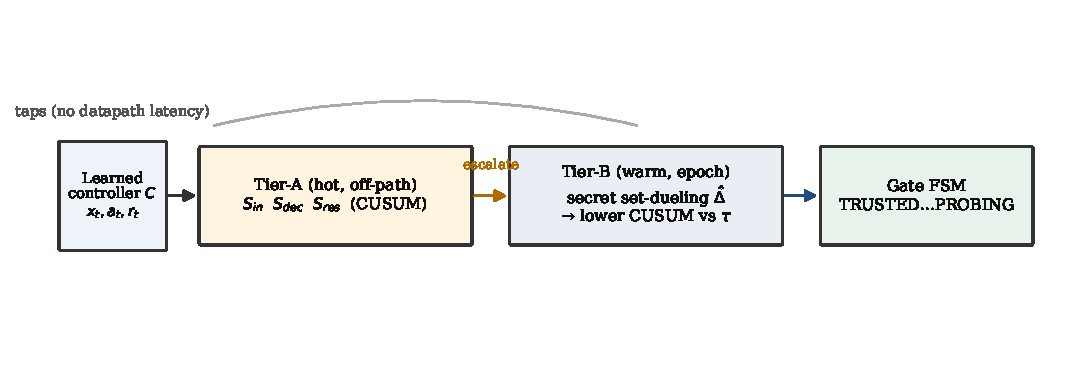
\includegraphics[width=\columnwidth]{arch.pdf}
\caption{Two-tier auditor. Always-on Tier-A tripwires raise the duty cycle of the
Tier-B competence confirmer. The estimator and gate logic are epoch-grained; the
per-access pool-tag lookup and output multiplexer remain (\Cref{sec:overhead}).}
\label{fig:arch}
\end{figure}

\textbf{Gate state machine.} A four-state finite-state machine (FSM) determines
where $C$ runs.
\emph{TRUSTED} runs $C$ everywhere and Tier-B at a low background duty cycle; a
Tier-A cumulative-sum (CUSUM) detector can move it to \emph{SUSPECT}.
\emph{SUSPECT} still runs $C$ everywhere but raises Tier-B's duty cycle; a Tier-B
alarm moves it to \emph{GATED}, while $T_{clear}$ clear windows restore TRUSTED.
\emph{GATED} runs $\pizero$ except on Leader-L, preserving a measurable $\dhat$,
and freezes online learning. After $T_{dwell}$ windows it enters \emph{PROBING},
which re-enables $C$ only on a small secret audited region. PROBING restores TRUSTED
after $T_{reprobe}$ estimates satisfy $\dhat\ge\tau+\Delta_{hys}$; otherwise it
returns to GATED with exponential dwell backoff. The entry threshold $\tau$, exit
threshold $\tau+\Delta_{hys}$, and minimum dwell prevent thrashing and make re-trust
measured rather than timer-based.

A design subtlety the build surfaced (\Cref{fig:fsm}): a \emph{pure} mimicry
attack keeps Tier-A silent, so if SUSPECT were the only route to GATED the attack
would evade the gate. We therefore allow the background Tier-B CUSUM to drive
TRUSTED $\to$ GATED directly; Tier-A escalation only \emph{accelerates} detection
by raising Tier-B's duty cycle. The two tiers trade latency/energy, not
correctness.

\begin{figure}[t]
\centering
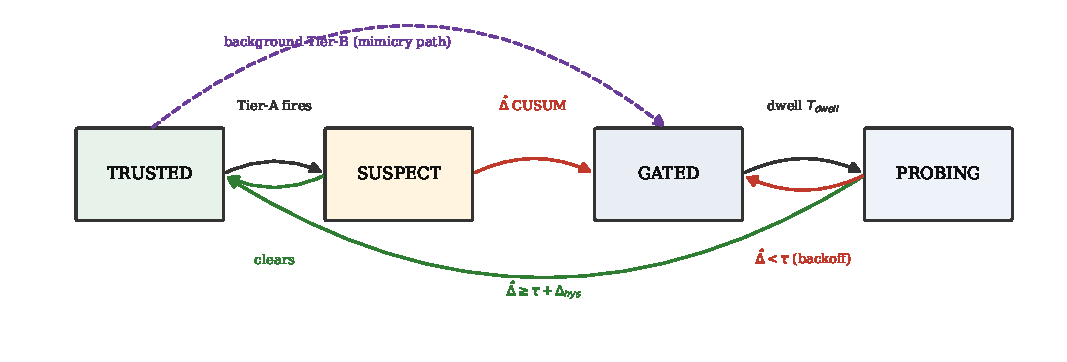
\includegraphics[width=\columnwidth]{fsm.pdf}
\caption{The trust-gate state machine. Hysteresis and a minimum dwell prevent thrash;
PROBING makes re-trust measured, not timed. The dashed path lets background
Tier-B gate a pure-mimicry attack that keeps Tier-A silent.}
\label{fig:fsm}
\end{figure}

\section{Tier-B: competence via randomized-secret set-dueling}\label{sec:tierb}
\textbf{Mechanism.} Partition the controller's resource (cache sets, memory
banks, PC-hash buckets) into three pools, reseeded each epoch (a fixed-length run of decisions) from a hardware RNG (random-number generator) whose assignment is unobservable to software: \emph{Leader-L} ($n_L$ sets, always
run by $C$), \emph{Leader-F} ($n_F$ sets, always run by $\pizero$), and the
\emph{Follower} rest (run whichever leader currently wins---what the victim mostly
experiences). Set-dueling---racing two policies on small dedicated sample pools---is already in
silicon~\citep{qureshi2007dip,jaleel2010rrip}; Bouncer repurposes it from policy
selection to policy trust. The estimator is
\begin{equation}
\dhat_w = \bar r_{L,w} - \bar r_{F,w},
\end{equation}
the mean reward rate on the sampled $L$ and $F$ sets in audit window $w$. Because
Leader-L sets \emph{ran} $C$ and Leader-F sets \emph{ran} $\pizero$, $\dhat$ is a
\emph{measured}, non-counterfactual quantity.

\textbf{Concentration $\to$ detection latency (the key tradeoff).} Suppose each
set contributes $m_{\mathrm{eff}}$ effectively independent bounded reward samples
per window, per-set means are uncorrelated within a pool, and the two pool means
are independent. Then
$\mathrm{Var}(\bar r_{\text{pool}})\le \rmax^2/(4m_{\mathrm{eff}}n)$, so
\begin{equation}\label{eq:var}
\mathrm{Var}(\dhat_w)\;\le\;\frac{\rmax^2}{4m_{\mathrm{eff}}}\Big(\tfrac{1}{n_L}+\tfrac{1}{n_F}\Big)
\;=:\;\sigd^2 .
\end{equation}
The i.i.d.\ synthetic harness has $m_{\mathrm{eff}}=m=64$; correlation reduces
$m_{\mathrm{eff}}$, and boundedness alone does not provide the $1/(mn)$ reduction.
To resolve a margin around $\tau$ one needs $\sigd$ smaller than that margin. Smaller
pools or shorter windows give a noisier $\dhat$, a higher CUSUM threshold $H$ to
hold the false-alarm rate, a longer detection delay $D$, and a larger safety-
floor slack (\Cref{lem:floor}). This chain---\emph{pool size $\to$ estimator
variance $\to$ CUSUM threshold $\to$ detection delay $\to$ regret floor}---is the
central design dependency; every hyperparameter lives on it.

\textbf{Detector.} Let $\gamma>0$ be a design margin and set the reference value
$K=\tau+\gamma/2$. A one-sided lower cumulative-sum (CUSUM) detector on $\dhat_w$
catches a downward shift below $\tau$:
\begin{equation}
C^-_w=\max\!\big(0,\,C^-_{w-1}+(K-\dhat_w)\big),
\end{equation}
alarming when $C^-_w>H$, and resetting on alarm (repeated CUSUM, so it re-arms
for the next change rather than latching after a long excursion). Standard
quickest-detection theory~\citep{lorden1971reacting,moustakides1986optimal}
motivates the CUSUM as the near-optimal detector for a downward shift under a
false-alarm constraint (optimality is exact only for a known post-change law;
here $\dhat_w$ is an estimated, variance-inflated statistic, so we treat it as a
well-motivated detector). \Cref{sec:guarantees} gives the average-run-length (ARL)
and delay constants.

\section{Tier-A: cheap tripwires}\label{sec:tiera}
Tier-A signals update on a sampled $1/k$ of decisions and \emph{never gate on
their own}: they only raise Tier-B's duty cycle. Their false positives therefore
cost confirmation work, not correctness. The released prototype uses the dense
statistics described below; \Cref{sec:overhead} reports an illustrative quantized
hardware budget rather than a synthesized implementation.

\textbf{$S_{in}$ (input covariate shift).} A frozen reference sketch of $D_{val}$
features: a random projection $P\in\mathbb{R}^{d\times p}$ ($p{=}8$) with the
projected validation mean and standard deviation. Online, it measures the squared
standardized displacement of the projected window mean. This statistic is
\emph{spoofable}---the adversary can hold its monitored marginals fixed---which is
why it cannot be the trust signal.

\textbf{$S_{dec}$ (decision-confidence collapse).} If $C$ exposes value/Q/logits,
monitor action-entropy collapse, max-$Q$ margin, and (for online learners)
temporal-difference-error magnitude (TD-error, the reinforcement-learning surprise signal). Pythia's reward and the confidence signals of SHiP and perceptron (two learned cache/branch controllers) are already computed in silicon~\citep{wu2011ship,jimenez2001perceptron}, so $S_{dec}$ is
nearly free there.

\textbf{$S_{res}$ (innovation residual).} A linear forward model
$g:(x_t,a_t)\to\hat r_t$ fit on $D_{val}$ ($d+2$ coefficients for the features,
action, and bias; $18$ at $d{=}16$); online residual $e_t=r_t-\hat r_t$;
two-sided CUSUM (a cumulative-sum drift detector) on $e_t$. This catches ``the world responds differently than at
validation'' even when input marginals look clean---the architectural analogue of
a Kalman innovation (the gap between a predicted and an observed signal). It is the signal that separates a competence-aware monitor
from an input-only one.

\section{Guarantees}\label{sec:guarantees}
\subsection{Safety floor / bounded regret}
\begin{assumption}\label{asm}
\textup{(A1)} Each normalized window reward lies in $[0,\rmax]$.

\textup{(A2)} A \emph{drop episode} is a maximal run of windows with
$\Delta_w<\tau$. During each episode, the expected number of \emph{fully-open}
windows---$C$ running everywhere in TRUSTED or SUSPECT, including the initial
detection delay and any false re-trust excursions---is at most $D$.

\textup{(A3)} The marginal false-alarm probability in each window is at most
$\alpha=1/\mathrm{ARL}_0$; no independence across windows is assumed.

\textup{(A4)} The total transient regret attributable to one false-alarm episode,
including all gate-state transitions it induces, is at most $c_{sw}$.

\textup{(A5)} A horizon of $T$ windows contains $N_{ep}$ drop episodes spanning
$T_{att}\le T$ windows.

\textup{(A6)} During a drop, the sets that keep running $C$ are chosen by the
secret sampler: the $n_L$ Leader-L sets always, plus in PROBING a uniform secret
follower subset of fraction $\rho_{aud}$, redrawn each epoch. Thus each set carries
$C$ with probability at most $\phi_P$, independent of its traffic ($\phi_G$ while
GATED and $\phi_P$ while PROBING).
\end{assumption}

A2 is an empirical assumption about the finite-state machine (FSM), not a
closed-form delay bound. \Cref{sec:eval-retrust} measures it through the implemented
controller. In the reseeded, near-i.i.d.\ harness, false re-trust is approximately
zero and $D$ is close to the initial-delay estimate $H/(K-\Delta_w)$. Temporal
correlation can inflate $D$; this temporal premise is distinct from the signed-mean
reseed-identifiability condition of \Cref{rem:stateless}.

\textbf{Audit exposure (from the construction).} A fixed slice of the resource keeps running the controller $C$ even during a drop, and this slice sets the audit-exposure cost. The $n_L$ Leader-L sets run $C$ in
\emph{every} gate state (they must, so $\dhat$ stays measurable and PROBING re-trust is
\emph{measured} rather than timed; \Cref{sec:tierb}), and PROBING additionally re-enables
$C$ on a \emph{uniform secret} fraction $\rho_{aud}$ of the followers---drawn by the same secret
sampler and redrawn each epoch, so a set's exposure does not depend on its index or traffic
(a fixed, e.g.\ sorted, audit subset would violate this; \Cref{sec:eval-floortraffic}). So the share of the resource still running
$C$ during a drop is $\phi_G=n_L/n_{sets}$ while GATED and
$\phi_P=\phi_G+\rho_{aud}\!\left(1-\tfrac{n_L+n_F}{n_{sets}}\right)$ while PROBING; at the pinned operating point these shares are small ($\phi_G{=}1.56\%$, $\phi_P{=}6.4\%$). Let $T_{att}$ be the
number of windows inside drop episodes.

\begin{figure}[t]\centering
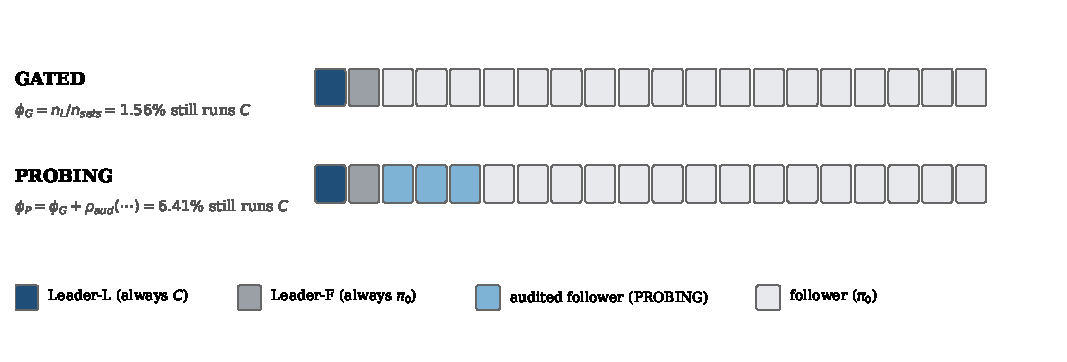
\includegraphics[width=\columnwidth]{exposure.pdf}
\caption{Which sets keep running $C$ during a drop (schematic, not to scale).
Leader assignments remain fixed within an epoch and are redrawn at the next.
GATED runs $C$ only on Leader-L ($\phi_G$); PROBING also runs $C$ on a uniform
secret follower subset ($\phi_P$ total exposure).}
\label{fig:exposure}
\end{figure}

\begin{lemma}[Safety floor, in expectation]\label{lem:floor}
Under \Cref{asm}, for an \emph{arbitrary} per-set traffic distribution, the expected regret
against the fallback---over the secret sampler, the detection delay, and the false-alarm
events---obeys
\begin{equation}\label{eq:floor}
\mathbb{E}\!\Big[\sum_{w=1}^{T}\!\big(\bar r_w^{\pizero}-\bar r_w^{\mathrm{Bouncer}}\big)\Big]
\;\le\; \underbrace{N_{ep}\,D\,\rmax}_{\text{detection + re-trust}}
\;+\; \underbrace{\phi_P\,T_{att}\,\rmax}_{\text{audit exposure}}
\;+\; \underbrace{\alpha\,T\,c_{sw}}_{\text{false alarm}}.
\end{equation}
The bound uses A1--A6 and linearity of expectation; its counting arguments require
only the marginal conditions in A2, A3, and A6, not independence across windows. The middle term
is the price of continuous, \emph{measured} auditability; it grows only at the dueling fraction
$\phi_P$ of the attack duration, not at full resource.
\end{lemma}
\begin{proof}[Proof sketch]
Partition windows and take expectations termwise.

\emph{(i) Audit exposure.} During a drop, Leader-L and the uniform secret
PROBING subset still run $C$. Their regret depends on the \emph{traffic} on those
sets, not their count. A hot set tagged for $C$ can therefore cost a full $\rmax$
in one window (\Cref{sec:eval-floortraffic}). Under A6, however, each set carries
$C$ with probability at most $\phi_P$, independent of its traffic. For any fixed
traffic vector $q$ with $\sum_s q_s=1$,
$\mathbb{E}[\text{exposure}]=\sum_s q_s\Pr[s\text{ runs }C]\rmax
\le\phi_P\rmax$. Summing over drop windows gives $\phi_PT_{att}\rmax$.

\emph{(ii) Detection and re-trust.} A2 counts every fully-open window in an
episode, including false re-trust excursions. Their expected regret is therefore
at most $N_{ep}D\rmax$.

\emph{(iii) False alarms.} By A3, the expected number of false-alarm episodes is
$\sum_{w=1}^{T}\Pr[\text{alarm}_w]\le\alpha T$; linearity suffices. A4 bounds the
total transient regret of each episode by $c_{sw}$.

\emph{(iv)} Windows in which the open controller outperforms the fallback
contribute non-positive regret. Summing (i)--(iii) proves \cref{eq:floor}.
\end{proof}

\textbf{A high-probability refinement, for exposure only.} This refinement uses
the released configuration in which one assignment epoch equals one audit window,
so A6 supplies a fresh uniform secret draw in every window. For a fixed sequence
of $T_{att}$ drop windows, let $X_w\in[0,\rmax]$ be exposure regret. Traffic may
adapt to gate history, so the $X_w$ need not be independent. Under A6, however,
$\mathbb{E}[X_w\mid\mathcal{F}_{w-1}]\le\phi_P\rmax$: the current secret draw is
uniform and independent of the past, and the input-only adversary is blind to it.
Thus $X_w-\mathbb{E}[X_w\mid\mathcal{F}_{w-1}]$ is a martingale difference whose
conditional range has width $\rmax$. Hoeffding--Azuma gives, with probability at
least $1-\delta_s$,
\begin{equation}\label{eq:floorhp}
\textstyle\sum_{w}(\text{exposure regret})_w \;\le\; \phi_P T_{att}\rmax \;+\; \rmax\sqrt{\tfrac{T_{att}}{2}\ln\tfrac1{\delta_s}},
\end{equation}
an $o(T_{att})$ slack that vanishes per-window over a sustained attack (empirically the envelope
covers the worst-case concentrated-traffic total with coverage $1.0$; \Cref{sec:eval-floortraffic}).
We do \emph{not} claim analogous high-probability forms for the detection and false-alarm terms:
the former would need a per-episode delay-\emph{tail} bound (A2 supplies only the mean) and the
latter a martingale/renewal concentration for the \emph{stateful} CUSUM (A3 supplies only the
marginal), neither of which we assume. The guarantee we assert is the expected-regret bound
\cref{eq:floor}.

\textbf{Two of the three regret terms are tunable, and one is fixed by design.} The detection and false-alarm slack are the \Cref{sec:tierb} knobs, while the
audit-exposure term is instead fixed by the design constant $\phi_P$. In the reseeded regime
where false re-trust $\approx0$ (\Cref{sec:eval-retrust}), A2's $D$ reduces to the initial delay
$D\approx H/(K-\Delta_{true})$, and the false-alarm rate is
$\alpha=1/\mathrm{ARL}_0$, where $\mathrm{ARL}_0$ (average run length to a false alarm) comes from Siegmund's corrected-
boundary approximation~\citep{siegmund1985sequential}, a standard sequential-analysis result. For a one-sided CUSUM (a running change detector)
accumulating $(K-\dhat)$ with standardized drift $\delta=(K-\mu)/\sigd$ and
boundary $b=H/\sigd+1.166$,
\begin{equation}\label{eq:siegmund}
\mathrm{ARL}(\delta)\;\approx\;\frac{e^{-2\delta b}+2\delta b-1}{2\delta^2}.
\end{equation}
In-control ($\mu\!\gg\!K$, $\delta\!<\!0$), $\mathrm{ARL}_0$ grows
\emph{exponentially} in $H/\sigd$, so false alarms are rare; out-of-control
($\delta\!>\!0$), the delay is short. The guarantee thus degrades gracefully and
\emph{quantifiably} with detection delay and false-alarm rate.

\subsection{Mimicry resistance}
We state the property \emph{conditionally}---it is exactly as strong as the
secrecy and the within-domain exchangeability it assumes, and we are explicit
that a \emph{global} $\dhat$ carries \emph{no} guarantee against a redistributive
attack.

\begin{proposition}[Mimicry resistance, per-domain]\label{prop:mimicry}
Fix a contested domain $R$, such as a victim's cache footprint. In every epoch,
draw Leader-L and Leader-F uniformly without replacement within $R$; the remaining
sets are followers, and the assignment is hidden from the adversary. Let
$\mu_{0,R}:=\mathbb{E}[\bar r_{F,R}]$ be the fallback pool's expected reward.
Assume that controller rewards on Leader-L and follower sets are exchangeable up
to a bias $|b_R|\le\beta$, and that the adversary holds aggregate Tier-A
statistics at their validation values.

\emph{(i) Expectation.} Any input-only strategy with
$\mathbb{E}[\dhat_R]\ge\tau$ satisfies
\[
\mathbb{E}[\bar r_{\mathrm{foll},R}^{C}]
\ge \mu_{0,R}+\tau-\beta .
\]
This is an unconditional expectation statement, not a guarantee conditional on a
single realized audit.

\emph{(ii) Sustained realized evasion.} Consider a block of $W$ windows. Assume
the $\dhat_{R,w}$ are independent conditional on the strategy and that
$W^{-1}\sum_{w=1}^{W}\mathbb{E}[\dhat_{R,w}\mid\text{strategy}]
\le\tau-\epsilon$. Fresh secret assignments alone do not imply this temporal
premise; gate-history-dependent reward processes can violate it. Because
$\dhat_{R,w}\in[-\rmax,\rmax]$, for any $W\ge2H/\gamma$,
\[
\Pr[\text{no alarm in the block}]
\le \Pr[W^{-1}\textstyle\sum_w\dhat_{R,w}\ge\tau]
\le e^{-W\epsilon^2/(2r_{\max}^2)} .
\]
\end{proposition}
\begin{proof}[Proof sketch]
\emph{(i)} Exchangeability gives
$\mathbb{E}[\bar r_L^C]=
\mathbb{E}[\bar r_{\mathrm{foll},R}^{C}]+b_R$. Since
$\mathbb{E}[\dhat_R]=\mathbb{E}[\bar r_L^C]-\mu_{0,R}\ge\tau$ and
$|b_R|\le\beta$, rearrangement proves the stated floor. Conditioning instead on
$\{\dhat_R\ge\tau\}$ would select favorable audit noise
(\Cref{sec:eval-prop1}).

\emph{(ii)} Hoeffding's inequality for independent, not necessarily identical,
variables of range $2\rmax$ gives the high-average bound
$e^{-W\epsilon^2/(2\rmax^2)}$. On a no-alarm block, no reset occurs and
\[
C_w=\max(0,C_{w-1}+K-\dhat_{R,w})
\ge\sum_{j=1}^{w}(K-\dhat_{R,j}).
\]
The strict alarm rule is $C_w>H$, so no alarm gives $C_w\le H$. At the end of
the block this implies
$W^{-1}\sum_w\dhat_{R,w}\ge K-H/W\ge\tau$ when $W\ge2H/\gamma$.
Thus the no-alarm event is contained in the high-average event.
\end{proof}

\textbf{Partial leakage (empirical scope).} The leak ablation uses a homogeneous
regional degradation model in which sparing a fraction $f$ of Leader-L sets
approximately removes the same fraction of degradation. At the operating point,
$\dhat_R\approx0.084<K$ at $f{=}0.6$ and $0.227>K$ at $f{=}0.8$, matching the
observed collapse in that band (\Cref{sec:eval-p4}). This is not a general
$f$-linear theorem: leaked sets could be a nonrepresentative subset of traffic or
harm.

\textbf{What this does and does not cover.} (i) \emph{Global $\dhat$ is not
enough.} A purely redistributive adversary that degrades the victim region while
holding the \emph{global} mean fixed evades a global $\dhat$ outright; only
per-domain dueling (the construction above, used in \Cref{sec:eval-p4}) detects
it. (ii) \emph{Heterogeneity bias.} Real cache sets / PC-buckets are not i.i.d.\
(hot/cold sets, conflict skew), so $\beta>0$; the guarantee degrades by $\beta$. Secret \emph{reseeding} each epoch shrinks this bias toward the i.i.d.\ value by
re-randomizing which physical cache sets act as leaders. (iii) \emph{Secrecy is
load-bearing.} The whole argument rests on the adversary being blind to the
within-$R$ assignment---which is why the secrecy ablation (\Cref{sec:eval-p4}) is
the headline experiment.

\textbf{The coverage hole (an explicit slow-bleed attack on the budget).} A
budgeted auditor has a finest resolvable competence drop. Let
$\rho:=n_{L,R}/|R|$ be the per-pool leader density, $k$ the chosen standard-error
multiplier, and $B$ the available per-pool leader budget. Under the effective-
independence premise of \cref{eq:var}, the within-$R$ resolvable gap is
$\delta_R=k\,\sigma_{\Delta,R}
=k r_{\max}/\sqrt{2m_{\mathrm{eff}}\rho|R|}$, requiring
$n_{L,R}\ge k^2r_{\max}^2/(2m_{\mathrm{eff}}\delta_R^2)$ leaders, independent of
$|R|$. A fixed budget $B$ therefore induces a finest
resolution $\delta_R^{\min}(B)$, and a redistributive adversary can pick a region
small enough (or trickle harm slowly enough) that its per-window competence drop
stays \emph{below} $\delta_R^{\min}(B)$ forever---an undeclared, sub-resolution
``coverage hole'' that the safety-floor lemma, proven only over the \emph{union of
audited domains}, does not bound. Finite resolution and assignment leakage are
distinct failure axes: the former hides small harm even with an intact secret,
whereas the latter lets an attacker spare audited sets. \emph{We therefore claim
mimicry resistance only for declared domains audited at resolution
$\delta_R^{\min}(B)$ with an intact secret---not general, any-region security}; the
slow-bleed attack is an open vulnerability. \Cref{fig:hole} demonstrates it
against the deployed auditor: constant per-window harm $h{=}0.06$ kept below
$\delta_R^{\min}$ bleeds a victim region for the entire horizon; cumulative harm
grows linearly as the horizon $T$ increases,
while the measured gap $\hat\Delta_R$ holds above the trust threshold ($0.205\!\ge\!\tau$) and the CUSUM (the cumulative-sum drift detector) never fires.

\begin{figure}[t]\centering
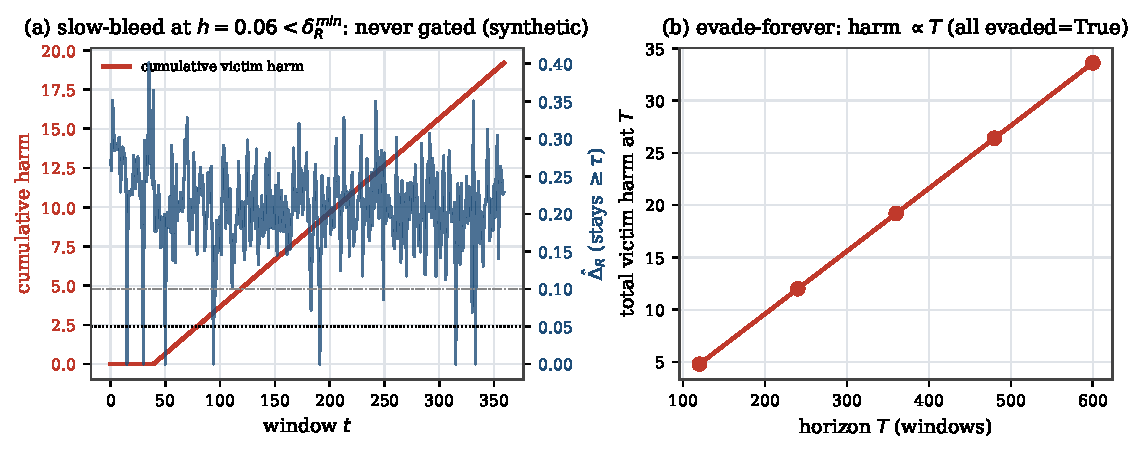
\includegraphics[width=\columnwidth]{coverage_hole.pdf}
\caption{The coverage hole, demonstrated (controlled harness, real Bouncer region
dueling). (a) a slow-bleed at $h{<}\delta_R^{\min}$ accumulates unbounded victim
harm while $\hat\Delta_R\!\ge\!\tau$ and no alarm fires; (b) it evades at every
horizon, so total harm $\propto T$. The closed-form floor is
$\delta_R^{\min}(B){=}k\sigma_{\Delta,R}\!\propto\!1/\sqrt{B}$ ($0.19,0.13,0.094,0.066$ for
per-pool leader counts $n_{L,R}{=}2,4,8,16$): more leader budget shrinks the hole
but never closes it.}
\label{fig:hole}
\end{figure}

\section{Attack-vs-drift triage}\label{sec:triage}
Attack and drift both trip the same failure test ($\Dw<\tau$, the audited competence margin falling below threshold), yet leave distinguishable signatures. Those differing signatures let us set the response prior (a secondary contribution---detection does not depend on it). Drift is
slower and phase-marker-correlated (tracking program-phase transitions) and is \emph{self-consistent} with a new-but-
valid regime (the forward model $S_{res}$ stays calibrated). An attack is abrupt,
can pulse, is \emph{targeted} at the decision boundary (high $S_{res}$ with small
$S_{in}$), and correlates with a specific co-tenant's schedule whose work yields
it no benefit except moving the shared $C$ (the contended shared resource). A small logistic model over the
auditor-observable $(\Delta S_{in},\Delta S_{res},|\nabla\dhat|,\text{co-tenant-
corr})$ suffices to separate the two. In the evaluation, probe P3 validates this triage model under cross-validation (holding out data to check it generalizes; \Cref{sec:eval});
misclassification only mis-selects between equally-safe responses.

\section{Per-controller instantiation}\label{sec:instantiation}
\Cref{tab:instances} maps Bouncer onto four controller classes, ordered by
\emph{set-locality}. \textbf{Cache replacement} leads: its hit/miss reward is
attributed to the set whose eviction it decided, giving the required spatial
attribution; representative sampling and reseed-identifiability are still needed.
\textbf{Branch/perceptron} predictors are indexed by program counter (PC), so the
decision and correctness reward are structurally local to a PC bucket, but
reseed-identifiability on real predictors is untested. \textbf{Prefetching} is
\emph{not} set-local---a prefetch on set $s$ rewards a different set $s'$, so the
faithful reward cannot be dualized (\Cref{sec:eval-champsim}); it is the
cautionary boundary. The \textbf{memory scheduler} is the hardest: no clean
set-sampling on a shared command bus to dynamic random-access memory (DRAM) forces
a \emph{model-based} $\dhat$, which
weakens \Cref{prop:mimicry}.

\begin{table}[t]\centering\footnotesize
\caption{Candidate controller instantiations. Set-locality asks whether a decision
and its reward share a dueling bucket; real-predictor reseed-identifiability remains
untested.}
\label{tab:instances}
\begin{tabular}{@{}lclll@{}}
\toprule
Controller & set-local? & $r_t$ proxy & fallback $\pizero$ & dueling resource\\
\midrule
Hawkeye/Glider (repl.) & \textbf{yes} & hit/miss & RRIP/LRU & cache sets\\
Perceptron branch & yes (PC) & correct & bimodal/gshare & PC slices\\
Pythia (RL prefetch) & \textbf{no} & acc.$\times$timel. & next-line/off & PC buckets\\
RL mem.\ scheduler & partial & $-$lat./$+$BW & FR-FCFS & banks/chan.\\
\bottomrule
\end{tabular}
\end{table}

\section{Methodology}\label{sec:method}
The formal results are conditional. Lemma 1 uses A1--A6; Proposition 1 additionally
uses within-domain representativeness and a temporal premise; estimator sizing in
\cref{eq:var} uses effective independence. Faithful attribution also requires
set-locality and reseed-identifiability (\Cref{def:setlocal,rem:stateless}). We map
each premise to evidence or assumption below rather than treating the environment
as irrelevant.

Controlled quantitative claims---latency, floor, mimicry survival, and secrecy---
come from one synthetic harness that satisfies these premises and is instantiated
three ways in P3. A separate ChampSim integration runs the auditor as a level-1
data-cache prefetcher and last-level-cache replacement module on SPEC\,CPU2017
traces. It is a real-simulator boundary study, not a full benchmark sweep
(\Cref{sec:eval-champsim}).

The harness uses $n_{sets}{=}2048$ sets and $m{=}64$ independent decisions per set
per window. An unobserved stress $u\in[0,1]$ drives drift and steering through
$\mu_C(u)=\rmax\,\mathrm{clip}(0.8-0.7u)$; the fallback is
$\mu_0=0.5\rmax$, or $q_0:=\mu_0/\rmax=0.5$. The map
$\mathrm{IPC}(\bar r)=0.6+1.4\bar r$ converts normalized reward to instructions per
cycle (IPC). \Cref{sec:eval-e3} varies both maps and $q_0\in[0.4,0.6]$; only the
tested qualitative behavior, not a universal transfer-function claim, is asserted.

The operating point is $n_L{=}n_F{=}32$, $m{=}64$
($|W|\approx1.3{\times}10^5$ decisions), $\tau{=}0.05$, $K{=}0.10$, and
$H{=}0.8$. At the boundary, CUSUM drift is $1.6\,\sigd$ on the background pool
($n_{bg}{=}8$) and $3.2\,\sigd$ at full duty ($n_L{=}32$). The R-latency sweep
therefore reports detection latency and fixed-deadline true-positive rate rather
than claiming deadline-free power (\Cref{fig:rlatency}). Conditions include clean
behavior, benign drift, and broad, mimicry, and regional attacks. Baselines are
no auditor, input out-of-distribution (OOD) monitoring through $S_{in}$,
oracle-$\Delta$, and always-fallback.

\textbf{Hypothesis discharge.} \Cref{tab:discharge} maps each premise to where it
is established, measured, or assumed. It also records which premises the
real-simulator studies do not satisfy.

\begin{table}[t]\centering\footnotesize
\caption{Hypothesis discharge: where each premise is established (E), measured (M),
or assumed (A). The harness satisfies the statistical premises by construction;
the real-cache study measures a reseed-identifiability failure.}
\label{tab:discharge}
\begin{tabular}{@{}p{0.30\columnwidth}p{0.62\columnwidth}@{}}
\toprule
Premise & Discharged \\
\midrule
A1 bounded reward $\in[0,\rmax]$ & E/M: synthetic by construction; real hit/miss $\in\{0,1\}$. \\
Representative within-domain sampling & A/E: equal $m$ per set in the harness; required, or replaced by traffic weighting, for $\dhat$ to target decision-weighted $\Delta_w$. \\
Effective independence for \cref{eq:var} & A/E: i.i.d.\ Bernoulli draws in the harness give $m_{\mathrm{eff}}=m$; correlated streams require a smaller effective sample size. \\
Prop.\ 1 within-domain exchangeability up to $\beta$ & A/E: assumed by the proposition; exact in the homogeneous harness and probed by the fixed cross-set heterogeneity sweep. \\
Reseed-identifiability of the contrast (\Cref{rem:stateless}) & A (synthetic: i.i.d.\ reward, holds by construction); \textbf{fails, measured, on a real cache} (\Cref{sec:eval-champsim}: reseeded $\dhat\!\approx\!0$ vs fixed-leader $0.23$). \\
A2 \emph{expected} fully-open windows/episode $\le D$ & A (assumed; $H/(K-\Delta)$ is a mean-delay approximation, not an upper bound); M: P1, R-latency, and false re-trust (\Cref{sec:eval-retrust}). \\
A3 marginal false-alarm prob.\ $\le 1/\mathrm{ARL}_0$ & A (assumed; \emph{approximated} by Siegmund's ARL, the mean run length between false alarms); M: P2 threshold operating points, sensitivity sweep. \\
A4 false-alarm-episode transient $\le c_{sw}$ & A (analytical accounting assumption). \\
A5 $N_{ep}$ episodes over $T$ & A (definitional, counts episodes). \\
A6 secret \emph{uniform} audit subset & E: construction (\Cref{sec:tierb}); M: PROBING exposure is $\phi_P$-uniform, index-independent (\Cref{sec:eval-floortraffic}: $0.062$/$0.064$ low/high index vs $0.985$ for a sorted prefix). \\
Prop.\ 1(ii) temporal premise (per-window $\dhat_R$ independent given the strategy) & A: holds in the synthetic harness (i.i.d.\ per-decision reward + fresh reseeds); \textbf{violable} by gate-history-dependent adversaries and correlated audits (\Cref{sec:eval-retrust}); \emph{not} inferable from reseeding alone. \\
Prop.\ 1 finite resolution $\delta_R^{\min}(B)$ & E under \cref{eq:var}'s effective-independence premise; M: sub-resolution slow-bleed (\Cref{fig:hole}). \\
Prop.\ 1 intact secret (leak $f{=}0$) & A in the proposition; M: homogeneous-degradation leak ablation, with collapse in the $f{=}0.6$--$0.8$ band. \\
\bottomrule
\end{tabular}
\end{table}

\section{Evaluation}\label{sec:eval}
The evaluation has four blocks. P0--P2 validate the estimator, causal gate, and
cost trade-off at the pinned synthetic operating point. P3--P4 test transfer
across synthetic controller abstractions and the constructed mimicry/leak
attacks. The following stress tests isolate assumptions and failure boundaries.
We finish with the formal regressions and the ChampSim boundary studies.

\subsection{P0: the estimator tracks ground truth}
The estimator $\dhat_w$ tracks the ground-truth competence gap $\Delta_w$ closely
as a benign drift carries competence from positive through zero to negative
(\Cref{fig:p0}(a)). The fit is $R^2{=}0.997$, with root-mean-square error
$0.0141\approx\sigd{=}0.0156$. This is a
\emph{controlled-harness} fidelity at the synthetic operating point ($m{=}64$); on
a real trace with far fewer samples per bucket the estimator is correspondingly
noisier (\Cref{sec:eval-champsim}). \Cref{fig:p0}(b)
checks the concentration bound \cref{eq:var} in the i.i.d.\ harness: across a pool-size sweep the
empirical std of $\dhat$ stays just below the bound at $0.85$--$0.98\times$ it, a tight upper
envelope (the bound uses $\tfrac14\!\ge\!p(1-p)$).

\begin{figure}[t]\centering
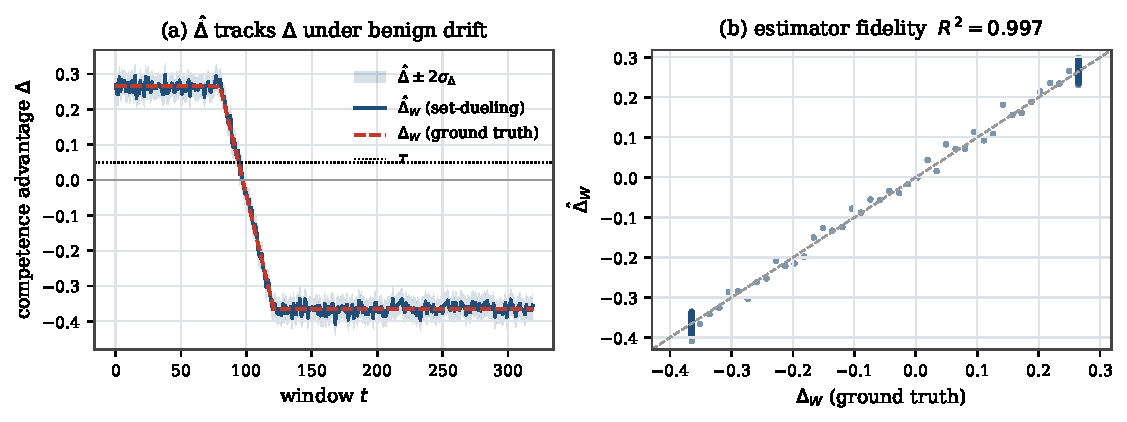
\includegraphics[width=\columnwidth]{p0_tracking.pdf}\\[2pt]
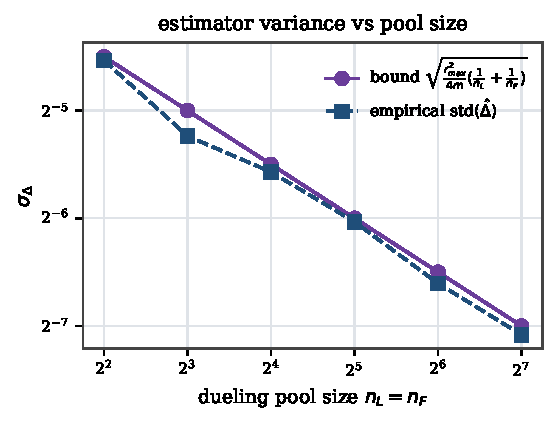
\includegraphics[width=0.62\columnwidth]{p0_variance.pdf}
\caption{P0. (top) $\dhat$ tracks ground-truth $\Delta$ ($R^2{=}0.997$);
(bottom) empirical $\mathrm{std}(\dhat)$ remains just below the variance upper
bound \cref{eq:var} in the i.i.d.\ harness.}
\label{fig:p0}
\end{figure}

\subsection{P1: detection, steady floor, and re-trust}
The attack begins at window 90 and ends at 200. The unguarded controller falls
well below the fallback, while Bouncer detects after \textbf{two} causally routed
audit windows and then uses $\pizero$. After the attack ends, PROBING re-trusts
$C$ after 15 windows; this recovery is measured rather than timer-only.

During attacked GATED windows, only the Leader-L fraction $\phi_G=32/2048$
continues to run $C$. The predicted mean IPC-floor violation is therefore
\[
  \phi_G\!\left(q_0-\mu_C^{att}/\rmax\right)
  \frac{1.4}{\mathrm{IPC}(q_0)}
  =0.579\%,
\]
where the injected stress is $u=0.92$, hence
$\mu_C^{att}/\rmax=\mathrm{clip}(0.8-0.7u)=0.156$; $q_0=0.5$; and
$\mathrm{IPC}(q_0)=1.3$. The measured attacked-GATED mean is $0.580\%$ and the
worst window is $0.64\%$. This is a mechanism calculation under the synthetic
IPC map, not a universal floor predictor.

The two pre-gate windows produce the larger transient dip ($36.5\%$ at its
worst). That cost belongs to the fully-open term in \Cref{lem:floor}. Once
gated, performance returns to $0.55$: the fallback floor, not clean performance,
because the attack removed $C$'s value. On clean input, the performance ratio is
$0.9965$; the permanent cost is the Leader-F sets that run $\pizero$.
The loose three-term expected-regret plug-in is $12.4$ IPC$\cdot$windows. The
smaller realized-gap/occupancy expression is reported later only as a descriptive
tracker, not as a bound.

Over the full clean--attack--recovery episode, cumulative regret ends at
$-69.48$ IPC$\cdot$windows: trusted operation captures enough of $C$'s clean
upside to more than repay the positive attack excursion. Keeping Leader-L on $C$
while GATED is the observability cost behind the residual exposure; parking those
sets on $\pizero$ would remove it but would also blind measured re-trust.

\begin{figure}[t]\centering
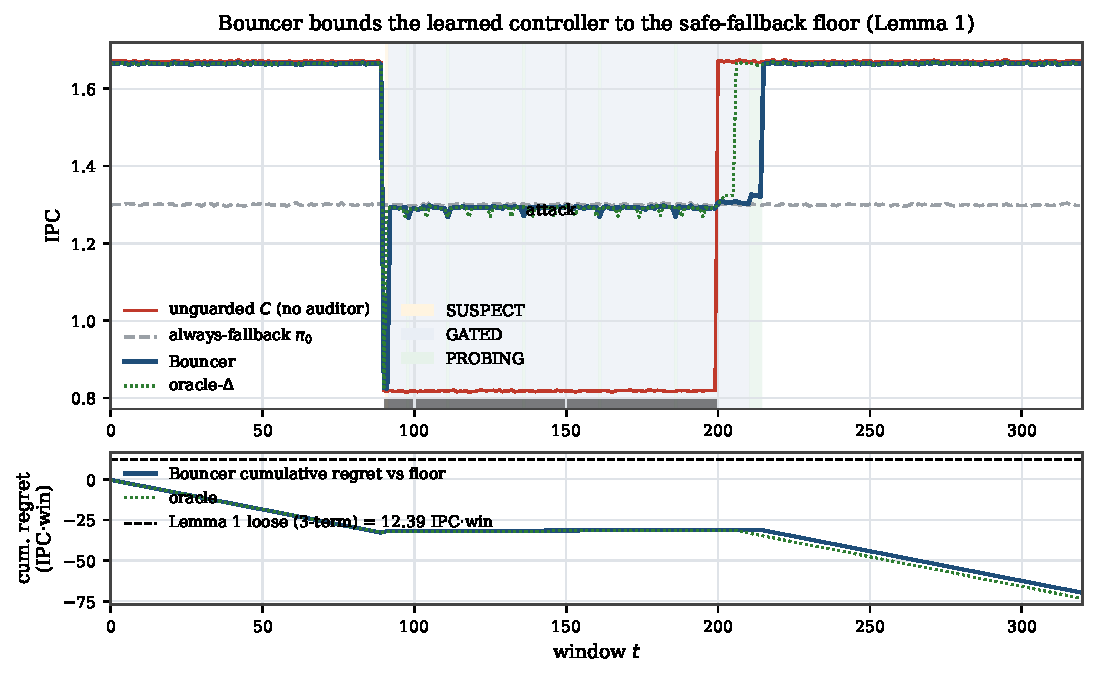
\includegraphics[width=\columnwidth]{p1_safety_floor.pdf}
\caption{P1. Bouncer bounds the controller to the fallback floor under attack and
re-trusts after it ends; the unguarded controller crashes below the floor.}
\label{fig:floor}
\end{figure}

\subsection{P2: ROC, the §\ref{sec:tierb} chain, and overhead}
The competence detector catches every tested attack while almost never firing on
benign episodes. \Cref{fig:p2roc} shows a true-positive rate (TPR) of $1.0$ at
false-positive rate (FPR) at most $0.05$ on the broad and constructed mimicry
attacks, while the
input-OOD detector $S_{in}$ works on the broad attack but collapses to
$\mathrm{TPR}{=}0$ under mimicry. Shrinking the dueling pool trades measurement noise for detection latency, tracking the analytic $D\!\approx\!H/(K-
\Delta)$. \Cref{fig:p2}(a) traces the
\Cref{sec:tierb} chain: as the pool shrinks from $128$ to $2$, $\sigd$ rises
$0.016\!\to\!0.125$, the calibrated $H$ rises $0.05\!\to\!0.35$, and detection
latency rises $0\!\to\!3.4$ windows. There is a clear knee near $n{\approx}8$: above it detection is
gap-limited and pool-insensitive, so larger pools only add overhead;
\Cref{fig:p2}(b) is the resulting overhead/latency Pareto frontier. The
illustrative 16-bit storage budget in \Cref{sec:overhead} is about $406$\,bytes, or
$0.155\%$ of a 256\,KB SRAM. It is not an RTL area, energy, or timing result.

\begin{figure}[t]\centering
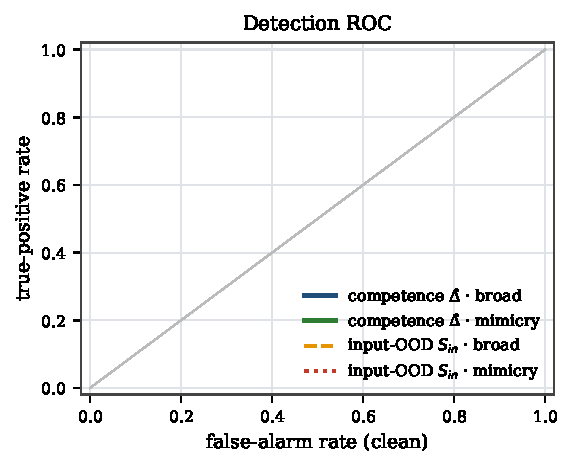
\includegraphics[width=0.78\columnwidth]{p2_roc.pdf}
\caption{P2 threshold-sweep operating points. Every tested threshold collapses
to the marked point: the competence detector catches broad and mimicry attacks;
$S_{in}$ catches only the broad attack. Coincident markers at $(0,1)$ are nested.}
\label{fig:p2roc}
\end{figure}
\begin{figure}[t]\centering
\begin{subfigure}{0.49\columnwidth}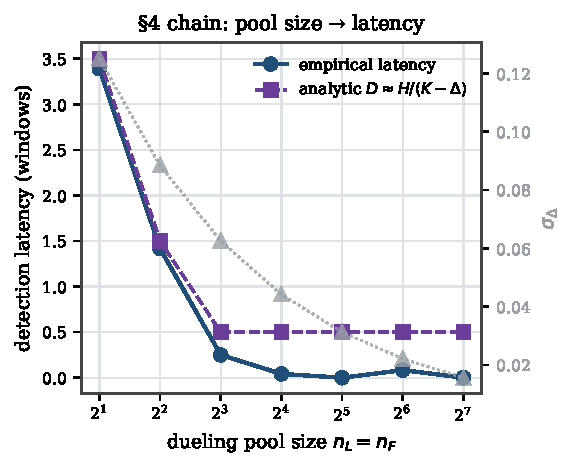
\includegraphics[width=\linewidth]{p2_latency_pool.pdf}\caption{}\end{subfigure}
\begin{subfigure}{0.49\columnwidth}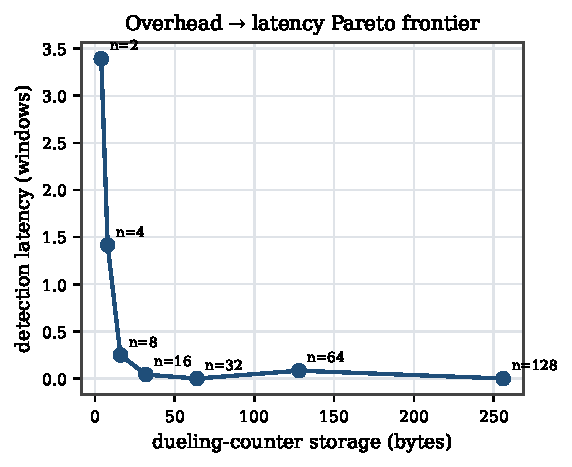
\includegraphics[width=\linewidth]{p2_overhead_pareto.pdf}\caption{}\end{subfigure}
\caption{P2. (a) pool size $\to\sigd\to H\to$ latency, with a knee near $n{=}8$;
(b) overhead/latency Pareto frontier.}
\label{fig:p2}
\end{figure}

\subsection{P3: synthetic controller abstractions and triage}
In the controlled harness, we instantiate the same auditor around abstract
prefetcher-, replacement-, and scheduler-like controllers (\Cref{fig:p3}, top).
The first two use secret set-dueling; the scheduler uses a model-based $\dhat$.
Across these abstractions, the steady-state floor violation remains at most
$0.7\%$ under broad attack and drift. The scheduler's weaker estimator increases
latency and does not inherit Proposition 1.

The constructed attack and drift episodes are also separable with
auditor-observable features (\Cref{fig:p3}, bottom). Five-fold cross-validation over
$120$ episodes reaches $100\%$ accuracy; abruptness is computed from estimated
$\dhat$, not ground truth. Accuracy remains $100\%$ when any one feature is
removed. This establishes separability in the evaluated synthetic episode family,
not general attack attribution.

\begin{figure}[t]\centering
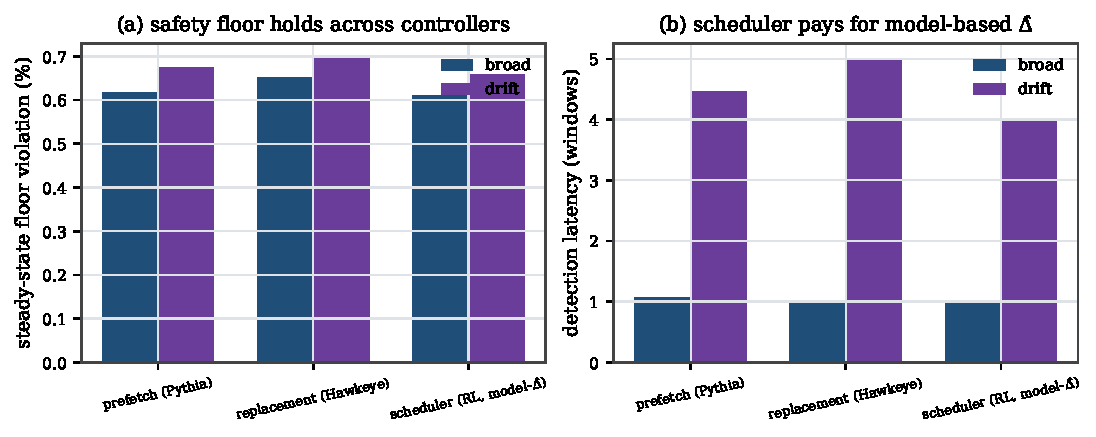
\includegraphics[width=\columnwidth]{p3_generality.pdf}\\[-1pt]
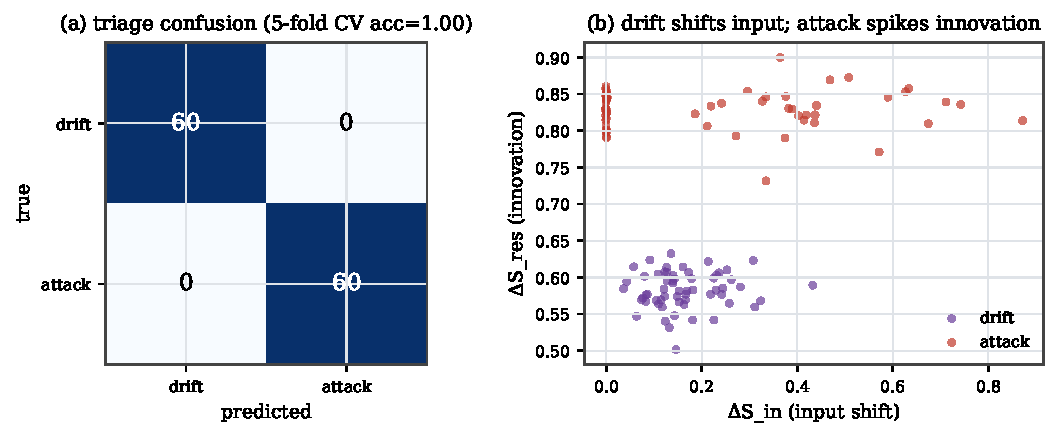
\includegraphics[width=\columnwidth]{p3_triage.pdf}
\caption{P3 synthetic abstractions. Top: the floor holds across three harness
instantiations. Bottom: attack and drift are separable within the constructed episode
family (five-fold accuracy $1.0$).}
\label{fig:p3}
\end{figure}

\subsection{P4: mimicry survival and the secrecy ablation}\label{sec:eval-p4}
\textbf{Competence versus input monitoring.} The mimicry adversary holds
$S_{in}$ in-distribution while degrading $C$. At each tested strength, the
input-OOD baseline detects $0/40$ episodes and full Bouncer detects $40/40$, with
$0/40$ clean false alarms for both. The input monitor's failure follows from the
construction (\texttt{suppress\_features}); Bouncer's measured $40/40$ is the
empirical result. Across $50$ seeds, Bouncer's true-positive rate (TPR) is $1.0$
with Wilson $95\%$ interval $[0.93,1.0]$, versus input-OOD TPR $0.0$
with interval $[0,0.07]$. Both clean false-positive rates (FPRs) are $0.0$
$[0,0.07]$. Detection latency is $2.0$ windows $[2.0,2.0]$, steady floor
violation is $0.641\%$ $[0.638,0.643]$, and clean performance ratio is
$0.99653$.

\textbf{What secrecy adds.} The regional experiment approximates Proposition 1's
fixed, nonempty within-$R$ pools by intersecting global pools with $R$. This gives
about four in-region Leader-L sets; a resulting pool is empty with probability
$0.013$ per window ($0.027$ for either pool), in which case $\dhat_R$ is set to
zero. Under this approximation and homogeneous regional degradation, TPR is $1.0$
for leak fraction $f\le0.4$, $0.975$ at $f{=}0.6$, $0.075$ at $f{=}0.8$, and
$0$ at $f{=}1.0$; latency rises from $2.2$ windows to infinity. Thus panel (a)
isolates competence measurement, while panel (b) isolates secrecy in this tested
regional model. It is empirical evidence, not a proof of an $f$-linear leak law.

\begin{figure}[t]\centering
\begin{subfigure}{0.49\columnwidth}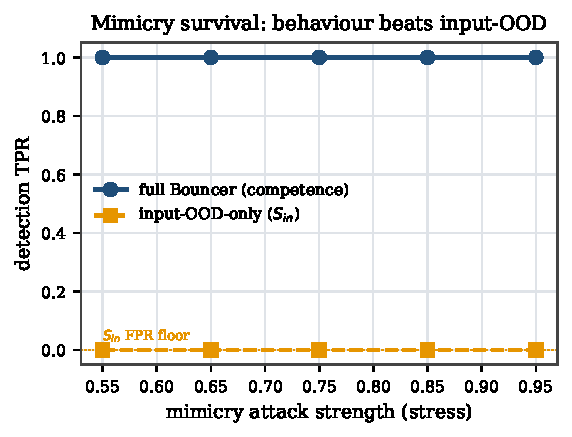
\includegraphics[width=\linewidth]{p4_mimicry_survival.pdf}\caption{}\end{subfigure}
\begin{subfigure}{0.49\columnwidth}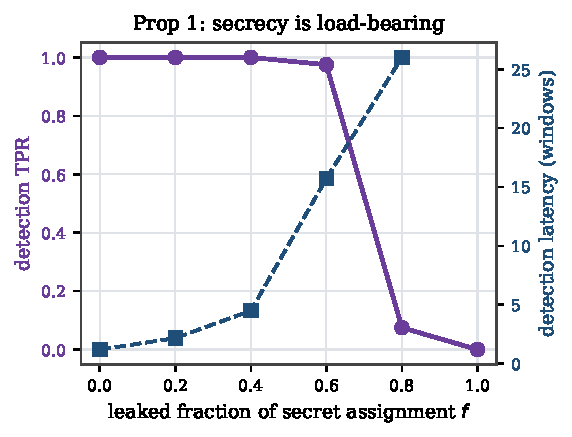
\includegraphics[width=\linewidth]{p4_secrecy_ablation.pdf}\caption{}\end{subfigure}
\caption{P4. (a) In the constructed mimicry attack, Bouncer detects every episode
while the input-OOD baseline is blind by construction. (b) Detection in the
homogeneous regional model collapses as the secret assignment leaks.}
\label{fig:p4}
\end{figure}

\begin{figure}[t]\centering
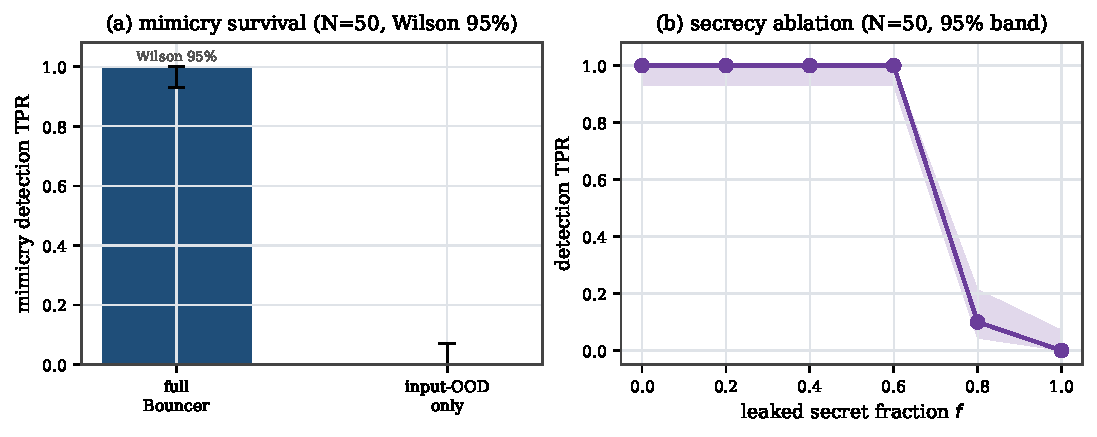
\includegraphics[width=0.49\columnwidth]{ci_mimicry.pdf}\hfill
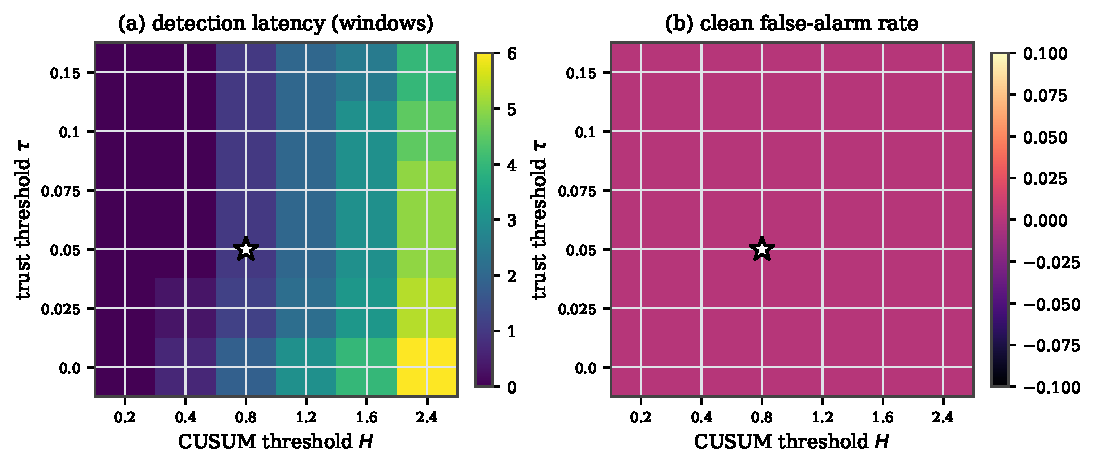
\includegraphics[width=0.49\columnwidth]{sensitivity.pdf}
\caption{Robustness. Left: headline results over $50$ seeds with Wilson 95\%
intervals. Right: sensitivity of detection latency and clean false-alarm rate to
$(\tau,H)$---the operating point ($\star$) sits on a broad plateau.}
\label{fig:ci}
\end{figure}

\subsection{Robustness: sensitivity and confidence}
The headline numbers are not single-seed artifacts (\Cref{fig:ci}, left; $N{=}50$,
Wilson 95\% intervals above), nor a knife-edge operating point: sweeping the trust
threshold $\tau$ and CUSUM threshold $H$ over a $6{\times}6$ grid
(\Cref{fig:ci}, right), most cells achieve $\le 3$-window detection with
clean FPR $\le 5\%$ and no missed episodes (\textbf{22/36})---a broad plateau around the
chosen $(\tau{=}0.05,H{=}0.8)$. Detection degrades gracefully and predictably
toward the plateau edges (small $H$ raises false alarms; large $\tau$ raises
misses), exactly as the \Cref{sec:tierb} chain predicts.

\textbf{Misspecification robustness.} Because the harness reward is built from the
theorems' assumptions (bounded reward, near-i.i.d.\ sets)---i.e., a reward specification that may not match reality---we test whether the
results survive violating them. We give each set a fixed competence offset
$\sim\mathcal{N}(0,\sigma_{het})$ (hot/cold sets, conflict skew), so Leader-C and
Leader-F pools are exchangeable only in expectation---the $\beta$-bias regime of
\Cref{prop:mimicry}. Sweeping $\sigma_{het}$ from $0$ to $0.30$
(\Cref{fig:robust}), mimicry detection stays at TPR $1.0$ and clean FPR at $0$,
the steady floor holds ($0.59$--$0.64\%$), and detection latency degrades only
gently ($2.0\!\to\!2.7$ windows)---because secret \emph{reseeding} re-randomizes
which physical sets are leaders each epoch, averaging the heterogeneity bias down.
This supports robustness to the tested fixed cross-set heterogeneity. It does not
test temporal dependence or remove the effective-independence premise of
\cref{eq:var}.

\begin{figure}[t]\centering
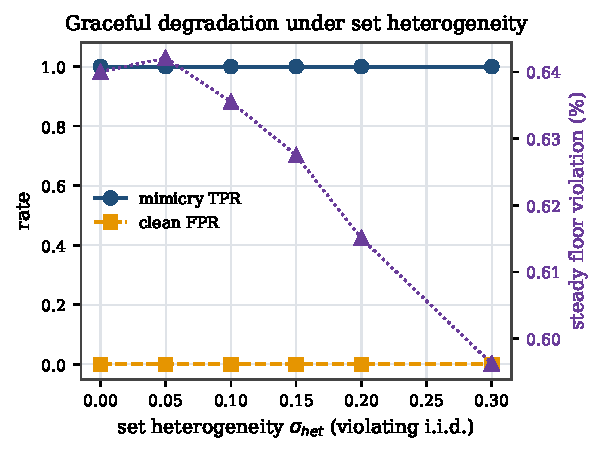
\includegraphics[width=0.62\columnwidth]{robust_env.pdf}
\caption{Graceful degradation when the i.i.d.-set assumption is violated: under
set heterogeneity $\sigma_{het}$ up to $0.30$, mimicry TPR stays $1.0$ and the
floor holds; detection latency drifts from $2.0$ to $2.7$ windows. Temporal
dependence is not varied.}
\label{fig:robust}
\end{figure}

\subsection{Reseed-identifiability: a stateful reward that stays auditable}\label{sec:eval-e3warmup}
\Cref{rem:stateless} predicts that a secret reseeded audit fails not on \emph{every} stateful
reward, but only when the policy \emph{contrast} depends on the state the reseed erases. We
isolate the two regimes on a predictor-like controller whose accuracy ramps with consecutive
windows on a policy (\Cref{fig:warmup}). With \emph{multiplicative} warmup
($\mathrm{acc}=\mu(1-e^{-ck})$, so the contrast scales with the warmup state), the secret
per-epoch reseed makes almost every sampled slice cold and $\dhat$ attenuates
from $95\%$ to $5\%$ of the fixed-leader estimate
($0.285\!\to\!0.015$ over $1/c{=}0.3\!\to\!20$ windows), while \emph{fixed}
leaders recover the full gap ($0.30$). With \emph{additive} warmup ($\mathrm{acc}=\mu-b e^{-ck}$,
contrast state-invariant at $0.30$), the reward is equally stateful yet the reseeded $\dhat$
\emph{survives} at $0.30$ ($\pm0.0015$) across the same warmup range---a stateful reward that
stays auditable, the direct counterexample to a statelessness \emph{requirement}. The
multiplicative case is the one that matches the ChampSim replacement study on one trace
(reseeded $\dhat{=}0.005$ vs fixed $0.23$). This is a \emph{synthetic} isolation of the
condition, not a real predictor: whether real PC-indexed rewards are reseed-identifiable at
window grain remains untested (\Cref{tab:instances}).

\begin{figure}[t]\centering
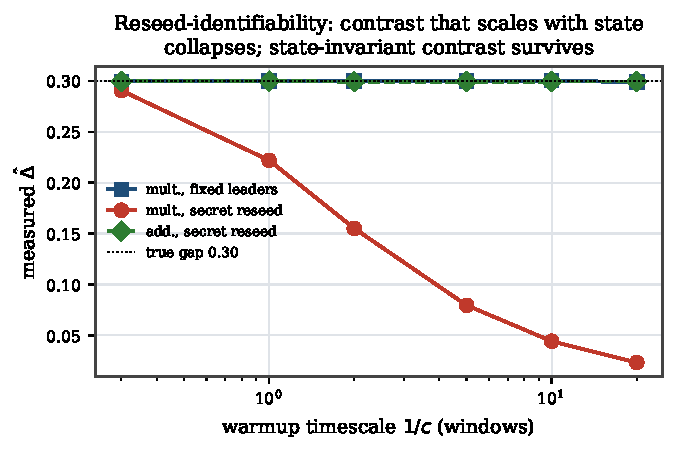
\includegraphics[width=0.62\columnwidth]{warmup_predictor.pdf}
\caption{Synthetic warm-up model. With a multiplicative warm-up contrast, secret
reseeding returns almost every sampled slice to the cold state and attenuates
$\dhat$; fixed leaders recover the $0.30$ gap. An equally stateful additive
warm-up with state-invariant contrast remains identifiable. This isolates a
mechanism; it is not evidence about real predictors.}
\label{fig:warmup}
\end{figure}

\subsection{Transfer-function sensitivity}\label{sec:eval-e3}
A reviewer's natural objection is that the headline percentages are artifacts of
the chosen controller-collapse curve $\mu_C(u)$ and IPC (instructions-per-cycle) map. We re-run the floor
(P1) and both P4 headlines across a family (\Cref{fig:e3}): the collapse curve as
$\mathrm{clip}$ and as a logistic at two slopes; the IPC map steeper and concave; a
\emph{joint} $\mu_C{\times}$IPC change; and---the load-bearing axis---the fallback
floor $q_0$ swept over $[0.4,0.6]$. \textbf{The qualitative guarantees are
invariant}: across every cell the steady floor violation stays $\le 0.9\%$ with a
genuine drop detected, mimicry TPR is $1.0$ for competence vs $0$ for the input-OOD
monitor, and the secrecy ablation keeps its TPR-vs-$f$ shape; only the exact
percentages move (clean tax $0.16$--$0.51\%$ across maps, on a reduced $20$-episode
budget per cell). Detection \emph{power} is the one quantity that is not constant. For \emph{any} genuine
off-policy episode ($\Dw<\tau$) the one-sided CUSUM (a sequential change detector) accumulates a drift
$K-\Dw\ge\gamma/2=0.05$, which at the boundary is $1.6\,\sigd$ on the background/TRUSTED pool
($n_{bg}{=}8$, $\sigd{=}0.031$) and $3.2\,\sigd$ only at full duty ($n_L{=}32$, $\sigd{=}0.016$)
after Tier-A escalation; per-domain audits see less. Every tested off-policy gap
gates within the 40-window horizon, but the quantity that actually varies is the
detection \emph{latency} $D\approx H/(K-\Dw)$, up to $H/(K-\tau)\approx 16$ windows at the
boundary, so the \emph{fixed-deadline} TPR falls as $\Dw\!\to\!\tau$. We measure this directly
(\Cref{fig:rlatency}): over eight true gaps, 40 episodes per gap, and 140-window
episodes with attack onset at window 20, the latency rises from
$2$ to $13.9$ windows tracking $H/(K-\Dw)$, and the by-$10$-window TPR drops from $1.0$ at a deep
drop to $0$ at $\Dw{=}0.04$ (recovering to $1.0$ by $20$ windows). Latency, not deadline-free
TPR, is the supported result. \emph{Scope:} this establishes robustness to the \emph{shape} of the
collapse curve, the IPC map, and the floor location; the Tier-A feature/confidence
maps are not swept (the headline competence-beats-input result is a Tier-B
property).

\begin{figure}[t]\centering
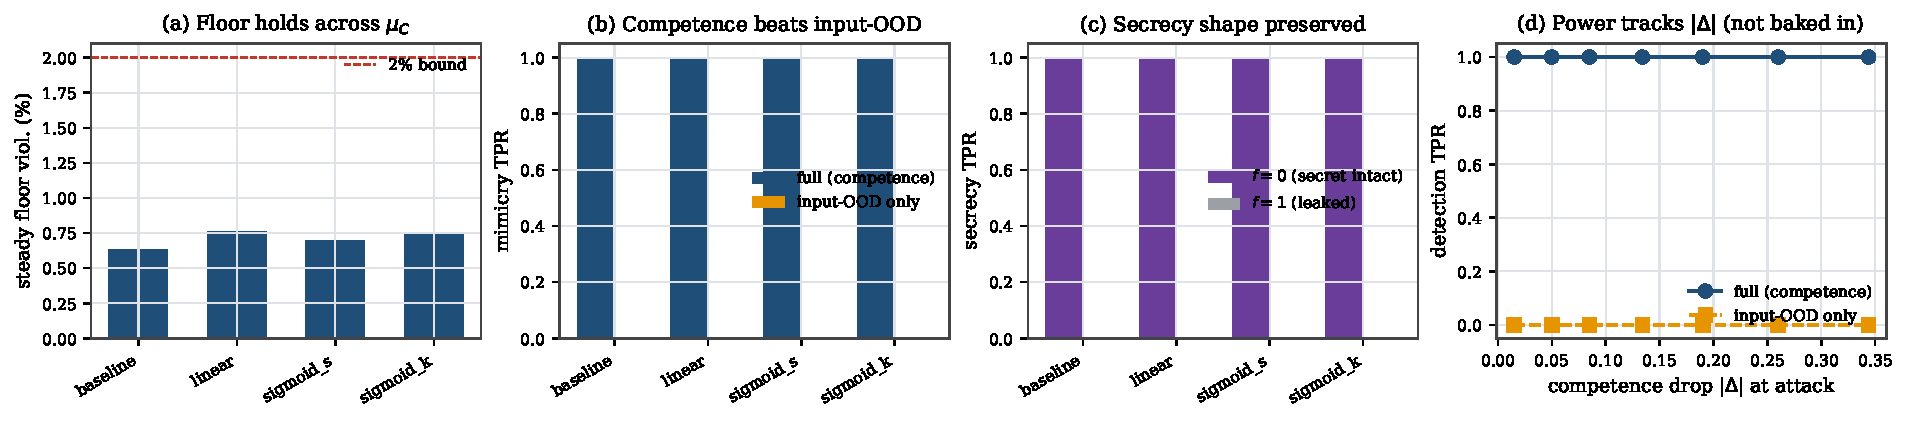
\includegraphics[width=\columnwidth]{e3_sensitivity.pdf}
\caption{Transfer-function sensitivity. Across the tested collapse-curve shapes (a), the
competence-beats-input mimicry result (b) and the secrecy-ablation shape (c) are
stable; (d) the competence detector gates on every tested off-policy gap
(within-episode TPR${=}1.0$ vs.\ input-OOD $0$), because the CUSUM drift $K-\Dw\ge1.6\,\sigd$
(background) throughout; what grows toward the $\tau$ boundary is the detection \emph{latency}
$D\approx H/(K-\Dw)$, so the fixed-deadline TPR falls (\Cref{fig:rlatency}).}
\label{fig:e3}
\end{figure}

\begin{figure}[t]\centering
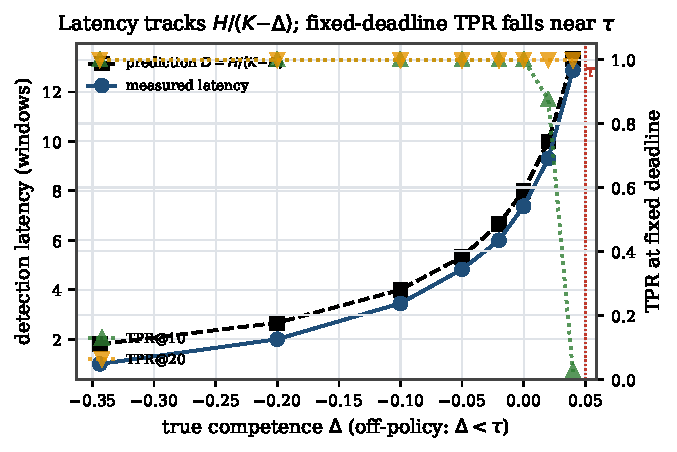
\includegraphics[width=0.62\columnwidth]{rlatency.pdf}
\caption{Detection latency vs.\ competence gap (positive form of \Cref{fig:e3}(d)). Every tested
gap gates within 40 windows (full-duty drift $3.8$--$28\,\sigd$;
$1.9$--$14\,\sigd$ background), but detection latency rises from $2$ to $13.9$
windows toward the $\tau$ boundary, tracking
the deterministic-drift limit $H/(K-\Dw)$, so the fixed-deadline TPR falls (TPR by $10$ windows
drops to $0$ at $\Dw{=}0.04$, recovering to $1.0$ by $20$).}
\label{fig:rlatency}
\end{figure}

\subsection{Adaptive timing adversaries}\label{sec:eval-adaptive}
Two timing-based evasions test threat-model completeness (\Cref{fig:adaptive}). \textbf{Boiling-frog}
(\Cref{fig:adaptive}, top): a very slow, stealthy degradation tuned to keep the
per-window change tiny. It cannot evade---a one-sided CUSUM (a running-sum change detector) integrates the
\emph{level} $(K-\dhat)$, not the slope, so once $\dhat<K$ it accumulates
regardless of how slowly it arrived. Bouncer gates $8$ windows after the true
$\Delta{<}\tau$ crossing (vs.\ $2$ for an abrupt attack); the slow descent only
\emph{delays} detection, and the steady floor still holds ($0.68\%$).
\textbf{PROBING-exploit} (\Cref{fig:adaptive}, bottom): a closed-loop attacker that
watches the audit's decision (its gate) and backs off during the GATED/PROBING states to pass the audit, resuming
when the TRUSTED state returns---the ``wait out the cooldown'' strategy. Because re-trust is
\emph{measured} (PROBING audits $\dhat$) and the dwell backs off exponentially,
the victim is harmed in $16.9\%$ of windows and the attacker spends $83.1\%$ of
the horizon backed off; there is no fixed cooldown to wait out. These are
finite-horizon measurements of this constructed strategy, not a general bound.

\begin{figure}[t]\centering
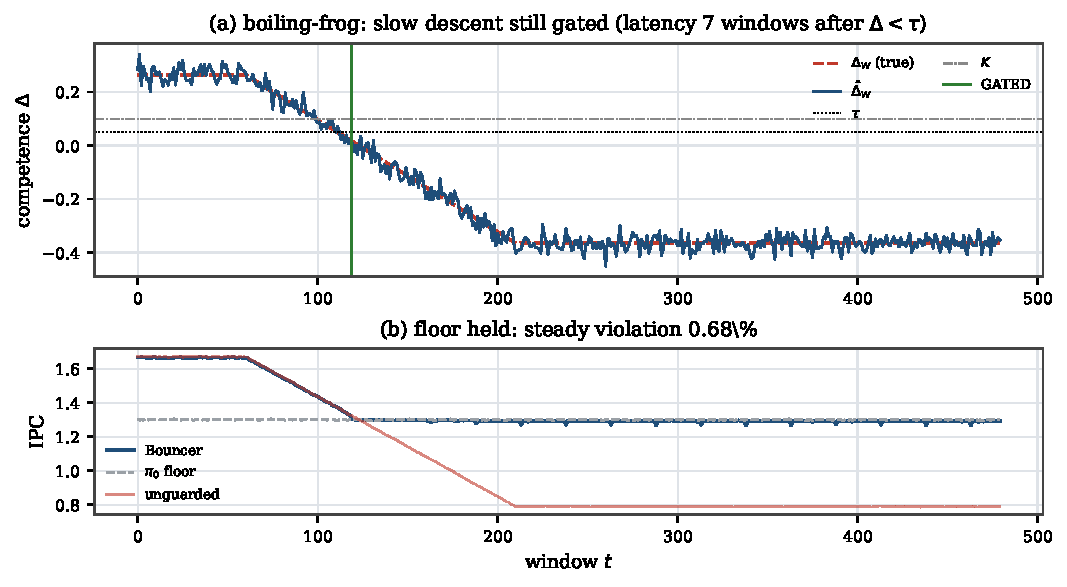
\includegraphics[width=\columnwidth]{adaptive_boiling.pdf}\\[-1pt]
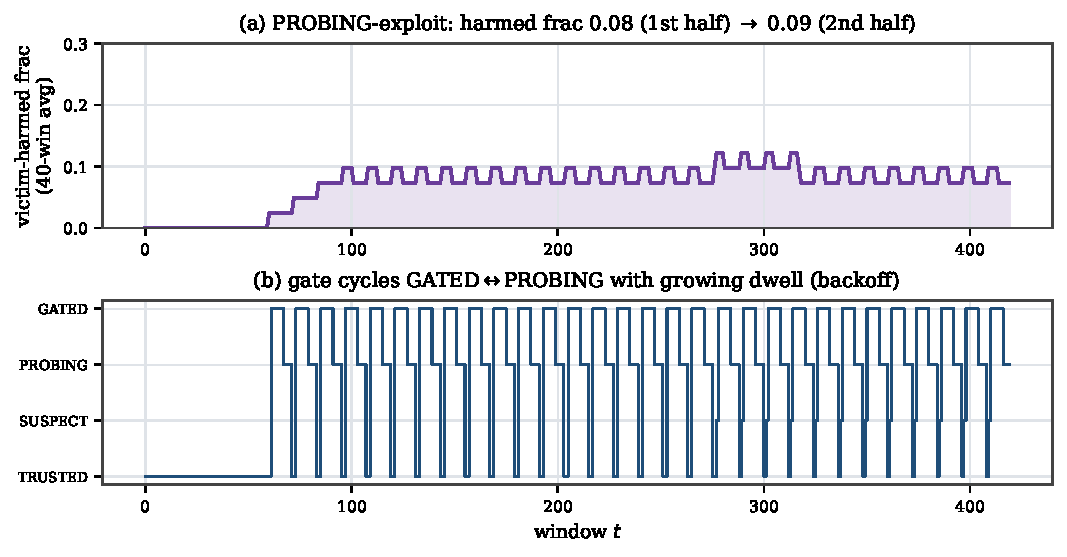
\includegraphics[width=\columnwidth]{adaptive_probing.pdf}
\caption{Adaptive timing adversaries. Top: boiling-frog is still gated (a CUSUM
integrates level, not slope). Bottom: the PROBING-exploit attacker is bounded to a small
harmed-window fraction ($16.9\%$) by measured re-trust and dwell backoff.}
\label{fig:adaptive}
\end{figure}

\subsection{Theory validation}
The top block of \Cref{fig:theory} checks the CUSUM constants on an i.i.d.\ Gaussian signal.
Across the threshold sweep, empirical average run length and detection delay
match Siegmund's approximation \cref{eq:siegmund}: the geometric-mean
empirical/theory ratio for $\mathrm{ARL}_0$ is $0.998$, and at $H=5\sigma$ the false-alarm run length
is 927 empirically versus 938 analytically. This is a formula sanity check. The
deployed synthetic operating point is in a stronger-drift regime, where
$H/(K-\Delta)$ is a useful mean-delay approximation.

The bottom block of \Cref{fig:theory} separates the proved loose form from a descriptive tracker.
For six short attack episodes, measured worst positive regret is $8.72$
IPC$\cdot$windows; the two-term expression is $15.14$, the realized-gap/occupancy
tracker is $9.48$, and the loose three-term plug-in is $47.42$. With three
episodes of length 960, audit exposure makes the two-term expression fail:
measured regret is $27.21$ versus $7.57$, while the tracker is $27.58$ and the
loose plug-in is $265.87$.

The persistent-drop regression is deliberately more adversarial. Across three
seeds, measured positive regret is $12.34$--$12.39$; the descriptive tracker is
$12.29$ and therefore slightly \emph{under-predicts}. The obsolete two-term
expression is $2.52$, while the loose three-term plug-in is $123.6$. We do not
call the tracker a bound: it combines realized occupancy and
gap with the approximate mean delay $H/(K-\Delta)$. The Lemma proves only the
loose expectation form under A2--A6. Its numeric instantiation remains
conditional on using the measured/assumed episode-level $D$; only the exposure
term has the separate high-probability envelope in \cref{eq:floorhp}.

\subsection{Traffic-weighted exposure}\label{sec:eval-floortraffic}
The audit-exposure term is traffic-weighted, and A6---a \emph{secret uniform} sampler---is what
bounds it in expectation. The released routing experiment establishes three
points. \emph{One-window concentration.} Put all of a window's traffic on one
hot set: the ordinary event that the sampler tags it Leader-L (probability $\phi_G$) makes the
entire window run $C$, so the realized one-window regret is $\rmax$---a $15.6\times$ violation of
the naive per-window $\phi_P\rmax$ allowance. This is why the bound must be an \emph{expectation},
not a per-window worst case. \emph{Why uniform sampling matters.} If PROBING audited a \emph{fixed}
(sorted-index) prefix of the followers, a low-index hot set would be exposed with probability
$1-n_L/n_{sets}=0.984$, not $\phi_P$---a $15.4\times$ violation of the \emph{expectation} that no
secrecy can fix. The released audit subset is instead a uniform secret
subset (\texttt{set\_dueling.is\_audited}), and a hot set's PROBING exposure is $0.062$ at low
index and $0.064$ at high index, both $\approx\phi_P{=}0.064$ and index-independent (versus
$0.985$/$0.017$ for the sorted prefix). \emph{Horizon-level concentration.} With the uniform sampler the
expected per-window exposure is $\le\phi_P\rmax$ for \emph{any} traffic (measured per-window mean
$0.064$ under worst-case concentration), and over independently reseeded windows the exposure
total stays under the Hoeffding envelope $\phi_P T_{att}\rmax+\rmax\sqrt{(T_{att}/2)\ln(1/\delta_s)}$
(empirical coverage $1.00$ at $\delta_s{=}0.01$ for every $T_{att}\!\le\!480$).

\subsection{Fully-open windows per episode: what $D$ actually is}\label{sec:eval-retrust}
A2's $D$ counts \emph{all} fully-open ($C$-everywhere) windows in a drop episode---the initial
detection delay plus any \emph{false re-trust} excursions, where PROBING re-opens the gate after
$T_{reprobe}$ audit estimates above $\tau+\Delta_{hys}$. We measure $D$ \emph{through the real
controller} (\texttt{exp\_retrust.py} drives the actual Tier-B CUSUM and FSM, so re-gating pays the
true CUSUM delay, not a one-window surrogate---an error a reviewer caught in an earlier draft).
\emph{With the reseeded, near-i.i.d.\ audit} a sustained true drop yields $\approx\!0$ false
re-trusts across drop depths (the audit reads $\Delta<\tau$ and rarely strings together
$T_{reprobe}$ crossings), so the fully-open fraction is just the initial-detection/SUSPECT
transient---$0.025$ (deep) to $0.073$ (near $\tau$), and $D\approx$ the initial delay. This is
\emph{not} horizon-independent in general: a temporally-\emph{correlated} audit produces
runs of crossings, so false re-trust occurs and the fully-open fraction climbs with the correlation
$\rho$---$0.008$ at $\rho{=}0$ to $0.225$ at $\rho{=}0.95$, again through the real controller.
\emph{Noise disclosure:} that $\rho{=}0.95$ headline injects innovation noise $0.10$, which is
$3.2$--$6.4\times$ the harness estimator noise ($\sigd{=}0.016$ full duty, $0.031$ background); a
noise sweep at $\rho{=}0.95$ shows the fully-open fraction grows with amplitude and stays small at
harness-matched amplitudes, so the $0.225$ is a property of this \emph{constructed}
correlated/high-variance counterexample, not of the harness. Temporal independence is an
assumption \emph{distinct} from reseed-identifiability's signed-mean condition; we do not equate
them. We therefore state $D$ as a \emph{measured
assumption} (A2) for the reseeded regime and name the correlated-audit inflation as a
\emph{limitation}, not a bound---and every Lemma-1 numeric floor reported in this evaluation
uses $D\approx$ the initial delay. Those numerals are therefore \emph{conditional plug-in
illustrations} of \cref{eq:floor}---valid where re-trust $\approx0$ as measured here, with
$H/(K-\Delta)$ a mean estimate rather than an upper bound---not standalone worst-case bounds.

\subsection{Realized evasion is selection-biased; sustained evasion is not}\label{sec:eval-prop1}
\Cref{prop:mimicry}'s expectation and sustained-evasion forms are separated by a
selection effect. \emph{Counterexample.} Two exchangeable sets
with rewards $\{1,0\}$ randomly permuted, one secretly Leader-L, fallback $0.2$, $\tau{=}0.5$,
$\beta{=}0$: unconditionally $\mathbb{E}[r_L]{=}\mathbb{E}[r_{\text{foll}}]{=}0.5$ (the identity
holds), yet conditioned on a single window's realized evasion the follower always drew the $0$---
$\mathbb{E}[r_{\text{foll}}\mid\dhat_R\ge\tau]{=}0.000$ with $P(\text{evade}){=}0.50$, far below
the putative $0.7$ floor. Conditioning on evasion \emph{selects} the noise, so
the expectation statement does not imply a single-window realized floor. Over
$W$ independently reseeded windows, the probability that this construction's $W$-window average
$\dhat_R$ stays $\ge\tau$ decays under the Hoeffding envelope $e^{-W\epsilon^2/(2r_{\max}^2)}$
(range $2\rmax$; a $W{=}100$ Rademacher regression rejects the stronger,
incorrect range-$\rmax$ exponent by $84.8\times$)
($0.50\!\to\!0.04$ measured from $W{=}1\!\to\!16$ vs.\ envelope $0.88\!\to\!0.14$), which is
\Cref{prop:mimicry}(ii). The same regression exercises the implemented CUSUM:
a prefix-average-below-$\tau$ stream need not alarm within $2H/\gamma$, but it verifies the
no-alarm$\Rightarrow$block-mean containment both on random degrading streams and
\emph{exhaustively} over every path of a three-point reward support from three starting
statistics. The floating-point implementation reports $2{,}068$ no-alarm and $654$
boundary-touching paths; exact-rational arithmetic gives $2{,}094$ and $682$.
Floating-point rounding therefore removes 26 no-alarm paths, a conservative
difference; containment holds in both sweeps. An exact $C{=}H$ boundary path
correctly does not alarm under the strict-$>$ semantics. The regression also computes an \emph{exact}
(dynamic-program) no-alarm probability for an in-support two-point degrading stream
($0.0038$, matched by Monte Carlo on the detector and below the corrected envelope $0.726$).
\emph{Operating-point check.} At the pinned operating
point ($n_L{=}32$ sets, $m{=}64$ decisions, independent per-set rewards) the single-window
follower selection bias is $\approx\!0$ ($0.004$); the catastrophe requires cross-set
anticorrelation \emph{plus} a tiny pool, and the CUSUM integrates over windows regardless.

\begin{figure}[t]\centering
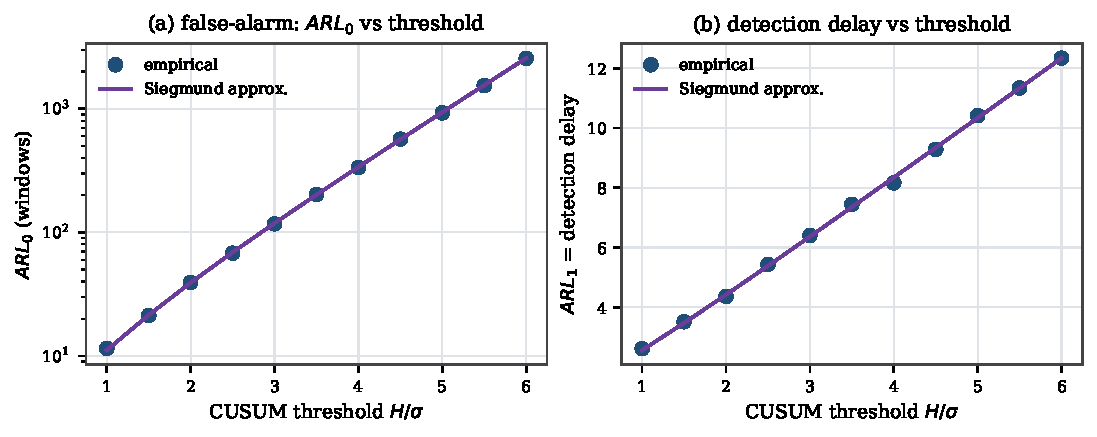
\includegraphics[width=\columnwidth]{th_arl.pdf}\\[-1pt]
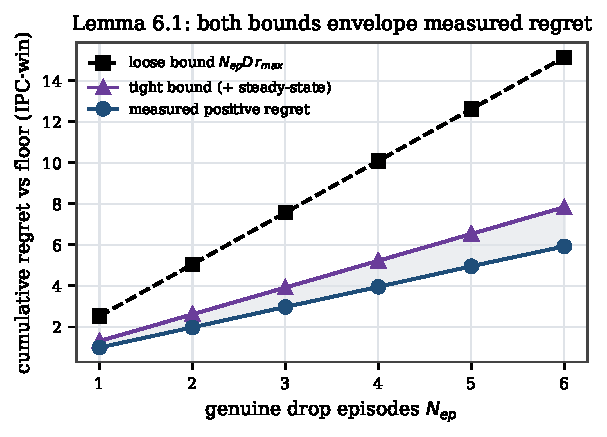
\includegraphics[width=0.62\columnwidth]{th_regret.pdf}
\caption{Theory. Top: ARL matches Siegmund. Bottom: measured regret versus the
two-term expression, loose three-term plug-in, and descriptive tracker.}
\label{fig:theory}
\end{figure}

\subsection{Real-systems integration: the set-locality boundary}\label{sec:eval-champsim}
The auditor compiles and runs in real ChampSim as \emph{both} a cache-replacement
module (set-local by \Cref{def:setlocal}---structurally the clean case, but
stateful; see below) and an L1D prefetcher
module (\emph{not} set-local). ChampSim is the standard trace-driven CPU cache simulator. The two together test the set-locality
\emph{boundary} on real program traces in ChampSim: the prefetcher case exhibits the
de-localization boundary in detail, and the replacement case shows the clean side
is set-local yet stateful---a second boundary (the secret reseed confounds a
path-dependent reward), rather than a real-hardware clean-case validation. We present the prefetcher case first because it is where the boundary
\emph{bites}---it is the cautionary result, not the headline.

\textbf{Prefetcher (the cautionary, non-set-local case).} We built a real
\textbf{ChampSim L1D prefetcher module}---the same set-dueling estimator, CUSUM,
and gate FSM C++ as \Cref{sec:overhead}---with the ``learned controller'' a
per-IP stride prefetcher, the fallback prefetch-\emph{off}, the reward the per-set
cache-hit rate, and the attack a cache-polluting corruption (the dueling
``sets'' here are virtual block-address buckets, $\mathrm{blk}\bmod 2048$, not
physical L1D sets). It compiles and runs
on SPEC\,CPU2017. The confirmer, CUSUM, reseed, and FSM execute off the
cache-access path at window granularity. A 2-bit pool-tag lookup and output
multiplexer remain per access; their RTL timing is not measured
(\Cref{sec:overhead}). The real $\dhat$ is far noisier than the
synthetic one, so we ran at a looser operating point (only $m\!\approx\!19$ accesses/bucket/window land, so $\dhat$
swings in $[-0.8,+0.7]$) ($\tau{=}0$,
$H{=}0.25$) than the synthetic $(\tau{=}0.05,H{=}0.8,m{=}64)$; we disclose this
rather than claim the synthetic $R^2{=}0.997$ estimator fidelity transfers (it
does not---that is a controlled-harness result).

\textbf{Across a three-trace suite (\Cref{tab:champsim}, \Cref{fig:champsim}) the
candid lesson is: the auditor is only as good as its competence reward.} The
\emph{floor cap is reliable}---on every trace Bouncer ends at the prefetch-off
floor, so the corruption attack's worst case is bounded: on streaming $619$.lbm a
corrupted prefetcher costs the unguarded config a large IPC hit ($7.9\%$, where IPC is instructions per cycle, a throughput measure) while Bouncer (already
at the floor) is unharmed; on compute-bound $600$.perlbench the attack is nearly
harmless ($0.3\%$) and so is the cap. But the per-set cache-hit reward
\emph{proxy} mis-estimates prefetch competence, so the clean tax ranges
$1.7$--$11\%$: on memory-bound $654$.roms stride prefetching genuinely helps IPC
($1.14$ vs the $1.01$ off floor), yet the hit-rate signal misses that benefit (it
comes from latency/MLP, not raw L1D hit count), so Bouncer over-gates. Two further
honesty points: the gate is \emph{competence}-driven, not attack-label-driven---on
lbm it engaged before the attack onset, so this is a floor cap, \emph{not}
attack-specific detection; and the TRUSTED$\to$GATED transition \emph{dynamics} are
shown where competence is controllable (the synthetic \Cref{fig:floor}), since no
available naive-prefetcher reward exhibits a clean pre-attack TRUSTED state here.

\begin{table}[t]\centering\footnotesize
\caption{ChampSim L1D suite (9M-insn SPEC). The floor cap bounds the attack on
every trace; the cache-hit reward proxy sets the clean tax.}
\label{tab:champsim}
\begin{tabular}{@{}lrrr@{}}
\toprule
SPEC trace & prefetch benefit & attack loss (unguard) & Bouncer clean tax\\
\midrule
600.perlbench (compute) & $+1.7\%$ & $0.3\%$ & $1.7\%$\\
619.lbm (streaming)     & $\approx\!0$ (hit-rate) & $7.9\%$ & $2.3\%$\\
654.roms (mem-bound)    & $+12.7\%$ & $5.2\%$ & $11.2\%$\\
\bottomrule
\end{tabular}
\end{table}

It is tempting to blame the hit-rate proxy and propose the controller's
\emph{own} reward as the fix---but we tested exactly that and it is
\emph{insufficient}. Holding $(\tau,H,\text{window},\text{partition},\text{FSM})$
fixed and swapping \emph{only} the reward, from per-set cache-hit to the
prefetcher's own accuracy$\times$timeliness, moves the roms clean tax only
$11.2\%\!\to\!9.7\%$ and still loses $5\%$ to the attacked-but-ungated prefetcher (single
trace, single seed; \texttt{hardening/experiments/N1\_reward\_swap/}).
The reason is a \textbf{fundamental tension in what set-dueling can measure}: the
cache-hit reward is \emph{set-local} (attributable to the dueling set) but a poor
utility proxy, whereas the own-accuracy reward is a faithful proxy but \emph{not
set-local}---a prefetch triggered on a Leader-L set targets a \emph{different}
address that lands on a \emph{different} set, so the dueling mis-credits it and
$\dhat$ collapses to $\approx\!0$. The dominant lever is therefore the
observation window / signal SNR, not reward fidelity: lengthening the epoch
(window $40\mathrm{k}\!\to\!200\mathrm{k}$) removes the over-gating even with the
crude proxy. This is a genuine limitation of set-dueling \emph{for prefetchers},
whose benefit is inherently de-localized; \emph{cache replacement}---where the
decision and its hit/miss outcome share a set---is set-local by construction (the
paper's ``home-turf'' condition): the structurally clean case in theory, though
\Cref{sec:eval-champsim} shows a real cache's stateful reward adds a second,
reseed-identifiability requirement before that cleanness is measurable. The milestone
this real-simulator boundary study sets up is accordingly sharper: a long-epoch, \emph{set-local} competence signal
(latency-weighted, replacement-style), not merely ``the controller's own reward.''

\textbf{Replacement (set-local but \emph{stateful}---a sharper boundary).} The same
auditor C++ compiles and runs as a real ChampSim \emph{LLC replacement} module:
DRRIP-style dueling on \emph{physical} cache sets (learned $C=$ an aggressive
LIP-style insertion, fallback $\pizero=$ SRRIP-HP) scored by the demand-hit reward.
Three real findings (\Cref{fig:e1repl}, $623$.xalancbmk), each of which
\emph{sharpens} rather than confirms the easy ``home-turf'' story.
\emph{(i) The prior ``$\dhat\!\approx\!0$'' was a software artifact, not sampling.}
A ChampSim replacement module's per-access hook fires only if the module also
provides a fill hook (\texttt{has\_cache\_fill}); without it the module sees
\emph{hits only}, the demand-hit reward collapses to $1$, and $\dhat$ is
\emph{identically} $0$. A cache fill is the insertion of a line on a miss, so without that hook the module never sees misses. Adding the fill hook makes $\dhat$ a real signal---so the
earlier null was a missing callback, not a horizon limit.
\emph{(ii) The whole-cache competence gap is real and large:} forcing every set to
the learned policy gives a far higher LLC hit rate than the fallback ($33.6\%$ vs $4.8\%$; LLC is the last-level cache).
\emph{(iii) Yet the secret per-epoch reseed---the very mechanism that buys mimicry
resistance---\textbf{confounds} the per-window estimate for this controller.} With
reseeding, $\bar r_L\!\approx\!\bar r_F$ and $\dhat$ sits at noise (clean mean
$0.005$) despite that $29$-point whole-cache gap; with \emph{fixed} leaders (reseed
off, DRRIP's own configuration) the \emph{same} estimator resolves it (clean mean
$\dhat\!=\!0.23$). The reason is that a replacement policy's reward is
\emph{path-dependent}: a set must run one policy \emph{consistently} to accumulate
the policy-specific cache state DRRIP's PSEL counter integrates, and reseeding each
epoch erases it. \textbf{Set-locality is thus necessary but not sufficient: a
secret, reseeded audit additionally requires a \emph{reseed-identifiable} policy
contrast} (a near-stateless reward is the clean sufficient case)---which the
synthetic harness's i.i.d.\ per-decision reward (A1) satisfies and a real cache,
whose contrast is path-dependent, does not at per-window grain. This is a genuine
secrecy/measurability tension, not a tuning issue: the clean-case competence and
transition dynamics consequently live in the synthetic harness (a faithful
\emph{stateless} set-local model, \Cref{fig:floor}), and the deployment milestone
is a reseed schedule slow enough to amortize cache-state warmup---a trade-off this
result makes precise.

\textbf{Disclosure (single trace, one seed).} The fixed-leader per-window $\dhat$ has std
$0.57$, so the resolution is a \emph{mean-level} effect: the clean mean $0.23$ is about $3$
standard errors over the $\sim\!50$ fixed-leader windows of one trace ($623$.xalancbmk). The
gate sat GATED in most clean windows of \emph{both} configurations ($84.6\%$ reseeded, $80.4\%$
fixed-leader), and the two committed logs follow different protocols ($82$ windows including
the attack for reseeded; $56$ clean-only windows for fixed-leader). A multi-trace replication
(\Cref{sec:disc}) is future work.

\begin{figure}[t]\centering
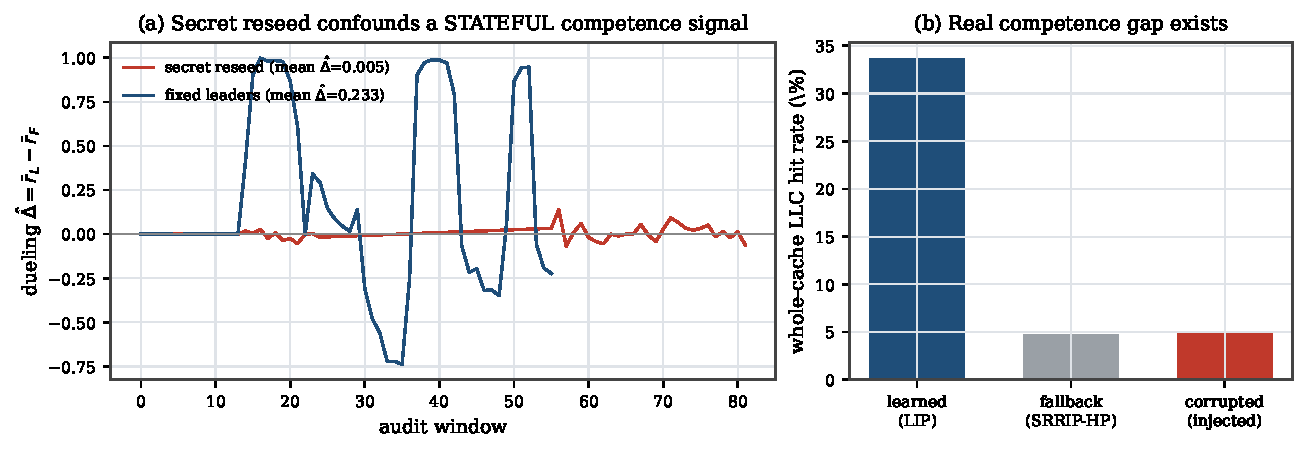
\includegraphics[width=\columnwidth]{e1_replacement.pdf}
\caption{Real ChampSim \emph{replacement} (623.xalancbmk). (a) The secret per-epoch
reseed---load-bearing for mimicry resistance---\emph{confounds} the per-window
competence estimate for a \emph{stateful} reward: with reseeding $\dhat$ sits at
noise; with fixed leaders the same estimator resolves the gap. (b) The whole-cache
gap is real (learned vs fallback); the \texttt{cache\_fill} fix makes $\dhat$
nonzero (it was identically $0$). Set-locality is necessary but not sufficient---a
secret, reseeded audit also needs a reseed-identifiable contrast. This is a boundary
result; the clean-case dynamics remain in the synthetic harness.}
\label{fig:e1repl}
\end{figure}

\begin{figure}[t]\centering
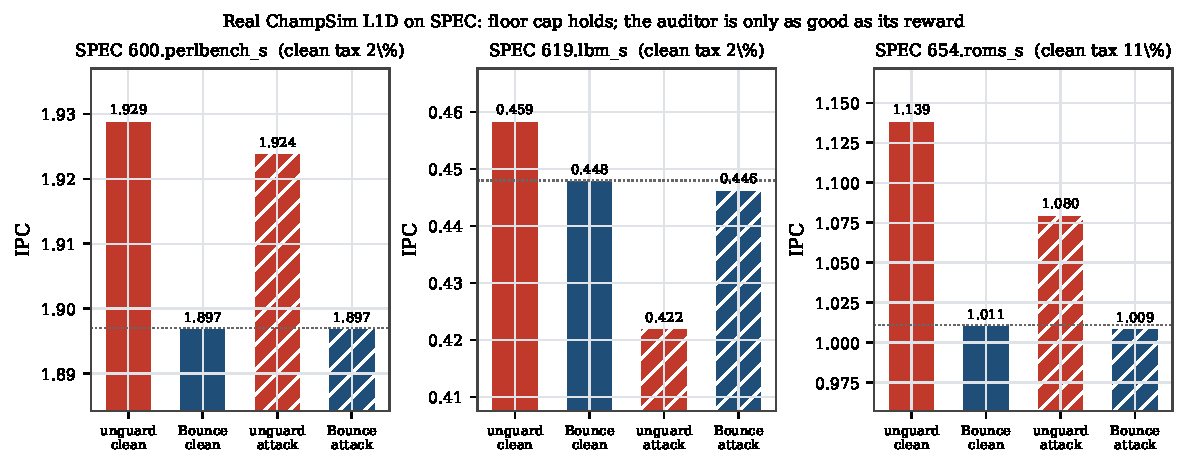
\includegraphics[width=\columnwidth]{champsim.pdf}
\caption{Bouncer as a real ChampSim L1D prefetcher across a SPEC suite. On every
trace Bouncer ends at the prefetch-off floor (the cap), bounding the corruption
attack's worst case (lbm: $7.9\%$ unguarded loss cannot reach the gated victim).
The per-set cache-hit reward proxy sets the clean tax ($1.7$--$11\%$): roms shows
the failure mode---a genuinely-helpful prefetcher under-credited and over-gated.
Swapping to the controller's own reward does \emph{not} fix this (only
$11.2\%\!\to\!9.7\%$); a prefetcher's benefit is not set-local, so set-dueling
needs a longer epoch or a set-local signal (replacement is the \emph{set-local}
case---though a real cache's stateful reward is a further boundary; see
\Cref{sec:eval-champsim}).}
\label{fig:champsim}
\end{figure}

\section{Overhead budget}\label{sec:overhead}
Table~\ref{tab:overhead} is an illustrative storage count, not a synthesized
implementation. It assigns 16 bits to each coefficient or reference statistic
and matches the released dimensions: a dense $16{\times}8$ projection plus eight
means and standard deviations for $S_{in}$; one confidence reference mean; 18
feature/action/bias coefficients plus one residual scale for $S_{res}$; three
two-sided Tier-A CUSUMs and one one-sided Tier-B CUSUM; and 64 set-dueling
counters. The total is about $406$ bytes, or $0.155\%$ of a 256\,KB SRAM.

The Python model uses floating point, so the numerical fidelity of this
quantization is untested. Dynamic energy, RTL area, and timing are also unmeasured.
The estimator, CUSUM, and FSM are architecturally off the access path, but the
per-access 2-bit pool-tag lookup and output multiplexer remain. Consequently we
claim an off-path organization, not a measured zero-latency result.

\begin{table}[t]\centering\footnotesize
\caption{Illustrative 16-bit storage budget; not synthesized.}
\label{tab:overhead}
\begin{tabular}{@{}lll@{}}
\toprule
Component & Storage & Per-decision work\\
\midrule
Set-dueling counters & 64\,B (reuse ATD) & reuse existing\\
$S_{in}$ dense projection + mean/std & 288\,B & 128 MACs on $1/k$\\
$S_{dec}$ reference mean & 2\,B & reuse confidence\\
$S_{res}$ model $g$ + residual scale & 38\,B & 18 MACs on $1/k$\\
CUSUM state: 3 two-sided + 1 one-sided & 14\,B & 1--2 add/cmp each\\
\midrule
\textbf{Total} & \textbf{406\,B} & estimator/gate off path\\
\bottomrule
\end{tabular}
\end{table}

\section{Related work}\label{sec:related}
\textbf{Learned microarchitectural controllers.} A growing body of work replaces hand-tuned heuristics with online or offline-trained predictors across every major structure Bouncer targets. RL memory schedulers \citep{ipek2008selfoptimizing} and RL prefetchers \citep{bera2021pythia} learn performance-coupled policies online; learning-based cache replacement imitates Belady's optimum with PC-indexed predictors \citep{jain2016hawkeye}, distilled neural models \citep{shi2019glider}, or signature-based hit predictors \citep{wu2011ship}; and neural and geometric-history branch predictors \citep{jimenez2001perceptron, seznec2006tage} have become the dominant adaptive prediction substrate. These designs share a failure surface: their advantage over a simple baseline (LRU/RRIP, a stride prefetcher, a bimodal predictor) is workload- and phase-dependent and can silently invert under distribution shift. Bouncer is agnostic to which of these controllers it wraps \emph{among the set-local, reseed-identifiable ones it can faithfully audit}; rather than proposing a new policy, it provides, for that class, the missing runtime guarantee that the controller costs, in expectation, no more than a small bounded amount over its own known-safe fallback.

\textbf{Set dueling and adaptive policy selection.} Set dueling \citep{qureshi2007dip} dedicates a handful of sampled sets to each of two competing policies and lets a single saturating counter steer the followers, a mechanism extended to re-reference prediction \citep{jaleel2010rrip}, shared-cache thread-aware insertion \citep{jaleel2008tadip}, and evicted-address filtering \citep{seshadri2012eaf}, and rooted in the sampling-monitor methodology of utility-based partitioning \citep{qureshi2006ucp} and sampling dead-block prediction \citep{khan2010sdbp}; a recent retrospective documents its industrial adoption and limits \citep{qureshi2007retro}. Bouncer borrows the dedicated-sets-plus-counter substrate but repurposes it from policy \emph{selection} to policy \emph{trust}: where DRRIP duels two heuristics to pick the empirical winner, Bouncer duels the learned controller against its fallback to \emph{certify} a competence advantage and, crucially, keeps the run-C/run-fallback assignment \emph{secret}. Classic set dueling assumes cooperative policies and is content to follow whichever wins; Bouncer must instead defend against a controller that may be steered or drifting, which is why its dueling sets feed a change detector and a trust gate rather than a preference counter.

\textbf{Safe RL, runtime assurance, and Simplex.} The closest architectural ancestor is Simplex \citep{sha2001simplicity}: a simple, formally verified safety controller bounds an unverifiable high-performance one via a decision module. Shielding \citep{alshiekh2018shielding} synthesizes a correct-by-construction shield from a temporal-logic specification, and constrained- and Lyapunov-based safe RL \citep{altman1999cmdp, achiam2017cpo, chow2018lyapunov, berkenkamp2017stability} keep policies inside a certified-safe set, with safe policy improvement \citep{thomas2015hcpi, laroche2019spibb} reverting to the data-collecting baseline wherever improvement is not statistically supported (surveyed in \citep{garcia2015survey}). Bouncer inherits the ``use simplicity to control complexity'' posture and the bootstrap-to-baseline reflex, but departs in what it must prove. Simplex and shielding require a \emph{verified model of the safety envelope}; constrained RL requires a known cost function. Bouncer needs neither: microarchitectural ``safety'' is not a state-space invariant but a relative performance floor, so it certifies only that the learned controller's \emph{realized reward} beats the fallback's on randomized dueling sets, with a bounded-regret safety floor (our Lemma) that holds without any reachability proof or verified plant model. The closest relaxation of Simplex's model requirement, Black-Box Simplex \citep{mehmood2022blackbox}, still forward-simulates a reachability/admissibility check and defines safety as a state-space invariant; Bouncer instead defines it as a measured relative-competence floor and needs no plant model at all. Concurrent runtime-assurance work certifies recovery \emph{deadlines} for adapting controllers via conformal prediction \citep{shojaei2026conformal}; Bouncer is complementary, certifying a competence floor rather than a recovery time, and adds the secrecy-based mimicry resistance that an observable certificate lacks.

\textbf{Change detection and OOD monitoring.} Tier-B runs a one-sided CUSUM
\citep{page1954cusum}, using quickest-detection theory
\citep{lorden1971reacting,moustakides1986optimal} and sequential threshold sizing
\citep{siegmund1985sequential,tartakovsky2014sequential}. Tier-A instead draws on
input monitoring: confidence baselines \citep{hendrycks2017baseline}, conformal
validity \citep{vovk2005algorithmic,lei2018distribution}, concept-drift detection
\citep{gama2014survey}, and representation-level shift tests
\citep{rabanser2019failing}. Such monitors measure whether inputs move; Bouncer's
duel measures whether realized controller reward falls relative to a fallback.

Related label-free deterioration tests include the Suitability Filter
\citep{pouget2024suitability}, sequential harmful-shift detection
\citep{amoukou2024sequential}, and D3M \citep{d3m2024}. Idealized D3M provides the
exact false-alarm guarantee; its practical variant approximately inherits it.
Bouncer's distinction is a secret, reseeded, hardware-oriented competence sample
with an expected-regret gate. The illustrative storage count is 406 bytes, but
the proposed quantization and RTL timing are unvalidated. Its attribution also
requires representative sampling, set-locality, and reseed-identifiability.

\textbf{Microarchitectural security and co-tenant attacks.} The controllers Bouncer audits are also attack surfaces. Contention and timing channels on caches \citep{osvik2006cache, yarom2014flushreload, liu2015llc, gruss2016flushflush} and occupancy channels \citep{shusterman2019occupancy} leak across cores and VMs in shared clouds \citep{ristenpart2009heyyou}, while branch predictors \citep{evtyushkin2016jumpoveraslr, evtyushkin2018branchscope} and prefetchers \citep{gruss2016prefetch, guo2022adversarialprefetch} expose secret adaptive state that an attacker can read out or steer. A learned controller widens this surface: its policy can be poisoned into amplifying leakage or into co-tenant denial of service. Prior defenses harden specific channels; Bouncer is orthogonal and complementary, bounding the \emph{aggregate} damage any steered controller can do by capping its cost at the vetted fallback. Its mimicry resistance (our Proposition) follows precisely from the secrecy of the set assignment, so an attacker who can observe and game stealthy counter-based detectors \citep{gruss2016flushflush} still cannot tell which accesses are being scored.

\textbf{ML-for-systems robustness.} Deployed learned components are brittle in exactly the regimes Bouncer guards. Oracle-imitation cache controllers lose accuracy off-distribution \citep{liu2020imitationcache}, learned indexes degrade on irregular data \citep{marcus2020benchmarklearnedindex}, and the Park benchmark documents why RL-for-systems policies behave unlike RL-for-games under noisy, non-stationary workloads \citep{mao2019park}; this is the hidden, system-level risk catalogued in \citep{sculley2015technicaldebt}. Production systems respond with bespoke guardrails: SLO-clamped colocation \citep{lo2015heracles}, OOM-bounded autoscaling \citep{rzadca2020autopilot}, and fault-triggered fallback in learned software \citep{carstens2023smartchoices}. Bouncer generalizes these one-off, fault- or threshold-triggered safeguards into a single hardware-cheap mechanism with a \emph{continuous} competence audit and a provable performance floor, applicable to any \emph{set-local, reseed-identifiable} learned microarchitectural controller rather than one tuned guardrail per deployment.


\section{Discussion and limitations}\label{sec:disc}
\textbf{Counterfactual cost.} Controllers without clean set-sampling (the memory
scheduler) force a model-based $\dhat$, which weakens \Cref{prop:mimicry}; we
scope sampling-friendly controllers first. \textbf{Redistributive mimicry and the
coverage hole.} A global $\dhat$ cannot see an attack that preserves the global
mean; per-domain dueling raises detection but does \emph{not} fully close it---a
slow-bleed adversary below the resolution floor $\delta_R^{\min}(B)$ evades
indefinitely (\Cref{prop:mimicry}, the coverage hole of \Cref{fig:hole}). We name
it rather than hide it.
\textbf{Ground-truth labeling.} ``Off-policy'' is operationalized as a sustained
competence drop beyond a fixed margin, against which we measure latency.
\textbf{Overhead vs.\ sensitivity.} The auditor dies if the Tier-B duty cycle is
too high; the minimal-overhead operating point---the knee of \Cref{fig:p2}(a)---is
reported as the result, not a footnote. \textbf{From simulation to silicon.} The
controlled quantitative claims are validated on a faithful harness. The real
ChampSim L1D module (\Cref{sec:eval-champsim}) shows the mechanism survives a
cycle-accurate simulator and bounds a corrupted prefetcher to the safe floor
across a 3-trace SPEC suite; a full SPEC/GAP sweep with a timeliness-aware reward,
and the production controllers of \Cref{tab:instances}, is the natural next step.
\textbf{Faithful attribution needs all three conditions.} Representative
within-domain sampling aligns the duel with deployed traffic; set-locality aligns
each decision with its credited outcome; and reseed-identifiability preserves
the policy contrast after leaders are shuffled. The per-set
cache-hit reward over-gates a genuinely helpful prefetcher on roms
(\Cref{sec:eval-champsim}, $11\%$ tax); swapping to the controller's \emph{own}
accuracy$\times$timeliness reward does \emph{not} fix it ($11.2\%\!\to\!9.7\%$),
because a prefetcher's benefit is intrinsically de-localized (it fetches a
different set than it was triggered on) and cannot be dualized to any per-set
reward. The structurally clean case is a controller whose decision and outcome
share a set---\emph{replacement}---a property of reward \emph{geometry} that
sharply scopes where set-dueling competence auditing is faithful.

\section{Conclusion}
Bouncer turns ``is the learned controller still earning its keep?'' into one
measurable scalar and bounds the cost of the answer. Its organizing result is the
\emph{set-locality} condition (\Cref{def:setlocal}): a secret per-set competence
audit can attribute reward to the policy that earned it only when a controller's
reward shares a set with its decision. That makes cache \emph{replacement} the
clean set-local case and prefetching the de-localized boundary. The real-systems
study adds a second condition: set-locality is necessary but not sufficient,
because a real cache is set-local yet \emph{stateful}, so the secret reseed that
buys mimicry resistance confounds its per-window measurement---a tension that a
\emph{reseed-identifiable} contrast resolves (\Cref{rem:stateless}).
Both controller-side conditions presuppose that the within-domain sample is
representative of deployed traffic, or is explicitly traffic-weighted.

For a controller in that class, Bouncer repurposes the set-dueling substrate into
a secret competence audit, gates an expensive confirmer behind cheap tripwires,
and proves a three-term safety floor---detection, audit-exposure, and
false-alarm---tied to the constants of the CUSUM detector. The payoff: for
declared domains audited at resolution $\delta_R^{\min}(B)$ with the secret intact,
Bouncer bounds the \emph{expected} competence regret, in the controller's own reward, against its
vetted fallback, under benign drift and an adaptive mimicry adversary alike, for
$406$ bytes in an illustrative 16-bit storage count. RTL area, energy, timing,
and quantized numerical fidelity are not evaluated. The robustness is
neither free nor unconditional: the competence signal is what beats an input monitor, and its
resistance to a \emph{leak-aware} attacker is purchased by the secrecy of the dueling sets---we
quantify the price of losing that secrecy, and we name the sub-resolution slow-bleed adversary
outside the audited domain as a real, un-closed vulnerability.

\section*{Broader Impact}
Bouncer is a defensive runtime monitor: it bounds the expected competence cost of a learned
microarchitectural controller against a vetted fallback, which serves a co-tenant denial-of-service
defense role in shared clouds. Two dual-use considerations. First, the secrecy of the reseeded
dueling assignment is what defeats a \emph{leak-aware} attacker (competence measurement is what defeats plain input mimicry); the same primitive could gate a shared
controller for censorship-style control, but the mimicry analysis (\Cref{prop:mimicry}) also
bounds what such gating can hide, since a global $\dhat$ cannot conceal a redistributive harm
from a per-domain audit. Second, we publish the sub-resolution slow-bleed coverage hole
(\Cref{fig:hole}) rather than hide it: naming the resolution floor
$\delta_R^{\min}(B)\propto 1/\sqrt{B}$ lets defenders budget leader counts against a target harm
rate, which we judge net beneficial because the attack is derivable from the public
concentration bound regardless. Online-weight poisoning is out of scope and stated as such
(\Cref{sec:threat}).

\section*{Reproducibility Statement}
All synthetic results, figures, and this PDF regenerate deterministically via
\texttt{./run\_all.sh} (CPython 3.11 with the versions pinned in \texttt{requirements.txt};
seeded RNG). \texttt{scripts/check\_paper\_numbers.py} (\texttt{run\_all} stage 9) is a
\emph{literal-presence audit}: it checks that headline numerals rendered from the released
\texttt{results/*.json} appear in the source. It is a regression tripwire for numeral drift, not
an exhaustive semantic audit of every claim. We check rendered strings rather than byte-identity
because floating-point results shift by $1$--$2$ ulps across numpy builds (the committed \texttt{hardening/manifests/} sha256 files are a
provenance record of one such build, not a portability claim). The harness invariants
(single-assignment-per-window; reseed) are checked by \texttt{experiments/test\_invariants.py}
(stage 0). The ChampSim figures in \texttt{run\_all} are regenerated from
committed JSON/CSV logs, not from a fresh simulator run.
\texttt{champsim\_plugin/setup\_champsim.sh} builds and runs the \texttt{lbm}
prefetcher case; \texttt{run\_e1\_replacement.sh} runs the single-trace
replacement case. Neither script regenerates the full three-trace suite in one
command. \Cref{lem:floor} has
two standalone regressions: \texttt{experiments/exp\_floor\_longattack.py} (the long-attack
audit-exposure envelope) and \texttt{experiments/exp\_floor\_traffic.py} (the traffic-weighting
counterexample and the expectation/high-probability repair).

\section*{Artifact Appendix}
The full artifact is released: the auditor and environment
(\texttt{bouncer/}), one script per evaluation phase (\texttt{experiments/}),
including the transfer-function sensitivity sweep
(\texttt{exp\_e3\_sensitivity.py}, \Cref{sec:eval-e3}), all result JSON and figures,
the real ChampSim L1D prefetcher \emph{and} LLC replacement modules
(\texttt{champsim\_plugin/bouncer\_pref/}, \texttt{bouncer\_repl/}), and the paper
source. \texttt{./run\_all.sh} regenerates every synthetic result, figure, and the
PDF (machine-dependent: $\sim$5 minutes on a fast laptop, $\sim$20 minutes in a constrained
sandbox; CPython 3.11, pinned numpy/scipy/matplotlib/pandas); all RNG is
explicitly seeded, so results are deterministic.
\texttt{champsim\_plugin/setup\_champsim.sh} clones and builds ChampSim, installs
the Bouncer module, fetches a public SPEC\,CPU2017 \texttt{lbm} trace, and runs
that prefetcher case; \texttt{champsim\_plugin/run\_e1\_replacement.sh}
reproduces the \Cref{sec:eval-champsim} replacement boundary study
(\Cref{fig:e1repl}) on \texttt{623.xalancbmk} (C++17 toolchain + vcpkg). The standalone auditor additionally builds with
\texttt{c++ -std=c++17 bouncer.cc -o bouncer\_selftest}.

\bibliographystyle{tmlr}
\bibliography{references}

\end{document}
